\pdfminorversion=4
\documentclass{beamer}

\usepackage{multicol}

\usepackage{bm} 
\usepackage{graphicx}
\usepackage{amsmath,amssymb}	
%Pour impression des transparents sans animations
%option trans (à préciser aussi dans les \only
%\documentclass[trans]{beamer}
%
%Pour impression des transparents sur papier (pour les CRR)
%\documentclass[handout]{beamer}
%


\newcommand{\procor}{\texttt{PROCOR}}
\newcommand{\inte}{\Gamma}
\newcommand{\fus}{\text{fus}}
\newcommand{\sol}{\text{sol}}
\newcommand{\cht}{\text{cht}}
\newcommand{\cond}{\text{cond}}
\newcommand{\chaL}{\mathcal{H}}
\newcommand{\vect}[1]{\bm{#1}}
\newcommand{\norm}{\vect{n}}
\newcommand{\gradGhost}{\overset{g}{\nabla}}
\newcommand{\difirho}{\frac{1}{\rho_l}-\frac{1}{\rho_s}}
\newcommand{\difrho}{\rho_l - \rho_s}
\newcommand{\npl}{{n+1}}
\newcommand{\nml}{{n-1}}
\newcommand{\ghost}{\overset{{g}}{\nabla}}
\newcommand{\entha}{\chaL}
\newcommand{\tim}{\mathcal{T}}
\newcommand{\refe}{\text{ref}}
\newcommand{\hlTab}[1]{\renewcommand{\arraystretch}{#1}}
\newcommand{\bord}{\text{bord}}
\newcommand{\subsubsubsection}[1]{\underline{\textit{#1}}}
\newcommand{\cell}{\text{maille}}
\newcommand{\som}{\text{som}}
\newcommand{\are}{\text{are}}
\newcommand{\maxi}{\text{max}}
\newcommand{\normeVec}[1]{\left\Vert #1\right\Vert}
\newcommand{\bib}[1]{{\color{cea_texte!80}\tiny\textit{[#1]}}}


\newcommand{\llb}{\llbracket}
\newcommand{\rrb}{\rrbracket}

\renewcommand{\frac}{\dfrac}

%%%%%%%%%%%%%%%%%%%%%%%%%%%%%%%%%%%%%%%%%%%%%%%%%%


\newcommand{\nn}{\nonumber}

\newcommand{\tx}[1]{{\text{#1}}}
\newcommand{\FF}[1]{{\mathsf{#1}}}
\newcommand{\FN}[1]{{\mathcal{#1}}}
\newcommand{\W}{\bm{W}}
\newcommand{\Wt}{\bm{\widetilde{W}}}
\newcommand{\tr}{\text{tr}}
\newcommand{\Frac}{\displaystyle\frac}
\newcommand{\Int}{\displaystyle\int}
\newcommand{\Sum}{\displaystyle\sum}
\newcommand{\matr}[1]{\mathbf{{#1}}}  
\newcommand{\dt}{\Delta t}
\newcommand{\dx}{\Delta x}
\newcommand{\dy}{\Delta y}
\newcommand{\dz}{\Delta z}  
%\newfont{\numerikEleven}{cmss11}
\newfont{\numerikEleven}{ecrm1000}
\newfont{\numerikTen}{cmss10}
\newfont{\numerikNine}{cmss9}
\newfont{\numerikEight}{cmss8}
\newfont{\numerikSeven}{cmss7}
\newfont{\numerikSix}{cmss6}
\newfont{\numerikFive}{cmss5}
\newfont{\numerikFour}{cmss4}
\newcommand{\ie}{\textit{i.e.} }
\newcommand{\aposteriori}{\textit{a posteriori }}
\newcommand{\apriori}{\textit{a priori }}
\newcommand{\ra}{\rightarrow} 
\newcommand{\lra}{\longrightarrow} 
\newcommand{\Lra}{\Longrightarrow} 
%\theoremstyle{plain}% Theorem-like structures provided by amsthm.sty
\renewcommand{\ell}{\begin{cursive}l\end{cursive}}
\newcommand{\egg}{\begin{cursive}lg\end{cursive}}

\renewcommand{\tx}[1]{{\text{#1}}}
\newcommand{\ext}{{\text{ext}}}
\newcommand{\intf}{{\text{in}}}

\newcommand{\liq}{{\text{liq}}}
\newcommand{\pool}{{\text{liq}}}
\newcommand{\ves}{{\text{ves}}}
\renewcommand{\top}{{\text{top}}}
\renewcommand{\bot}{{\text{bot}}}
\newcommand{\massEnthalpy}[2][\null]{h_{#2}^{#1}}

\newcommand{\Va}{{\textit{Cht. Vol. 1.0}}~}
\newcommand{\Vb}{{\textit{Cht. Vol. 2.0}}~}
\newcommand{\IBC}{{\textit{IBC}}~}
\newcommand{\hist}{{\textit{version 1.8.1}}~}




\newcommand{\bea}{\begin{eqnarray} }
\newcommand{\eea}{\end{eqnarray} }
\usetheme{cea2019}

%\usepackage[default,scale=0.85]{opensans} 
%\usepackage{lmodern} 



%
\titre{Modélisation et simulation numérique des fronts de fusion/solidification à l'interface d'un bain de corium}
\evenement{Soutenance de thèse}
\auteurs{Adrien Drouillet, CEA, IMB}
\datedocument{17 décembre 2021}
\auteurprincipal{Adrien Drouillet}
%%
\begin{document}

%% TITLE PAGE %%
\PageTitre{}
%%




\section{Contexte}
\begin{frame}
    \frametitle{Contexte accident grave de réacteur nucléaire}
\begin{columns}[c]
        \begin{column}{0.4\textwidth}
            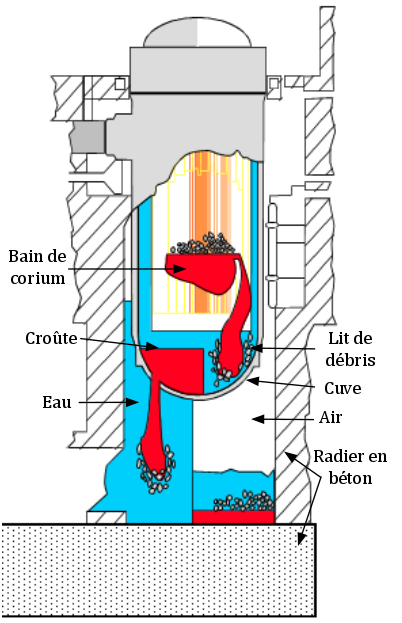
\includegraphics[width=0.9\textwidth]{Figures/accident_grave.png}
        \end{column}
\footnotesize
	\begin{column}{0.6\textwidth}
		\begin{ceablock}{Un accident grave de réacteur nucléaire}
			\begin{itemize}
				\item Mauvaise évacuation de l'\textbf{énergie thermique} produite par le cœur.
				\item Formation de \textbf{corium} (liquide composé des éléments du cœur fondu) par dégradation du combustible.
				\item \textbf{Propagation du corium} en cuve, puis potentiellement dans le puits de cuve. {\color{cea_texte!80}\tiny\textit{[Jacquemain et al.]}}
			\end{itemize}	
	    	\end{ceablock}
		\begin{ceablock}{Stratégies de rétention en cuve (IVR)}
		\hspace{-0.8cm}\\
		\underline{Objectif :} contenir le corium en cuve.
			\begin{itemize}
				\item \textbf{Tenue thermique} de la cuve.
				\item Tenue mécanique de la cuve.
			\end{itemize}	
	    	\end{ceablock}
		$\Rightarrow$ Étude de la thermohydraulique du bain de corium et de la fonte de la cuve.
        \end{column}
\normalsize
	\end{columns}
\end{frame}

\begin{frame}
    \frametitle{Physique du bain de corium}
    \scriptsize
    \begin{ceablock}{Principaux phénomènes}
        \begin{itemize}
		\item \textbf{Stratification du bain} en plusieurs phases immiscibles et de propriétés différentes. {\color{cea_texte!80}\tiny\textit{[Tsurikov et al.]}}
		\item Phénomène de \textbf{convection} dus aux forts gradients de température dans la partie oxyde.
		\item Phénomène de \textbf{focalisation des flux thermiques} au niveau de la couche mince.
	\end{itemize}
    \end{ceablock}
\begin{center}
		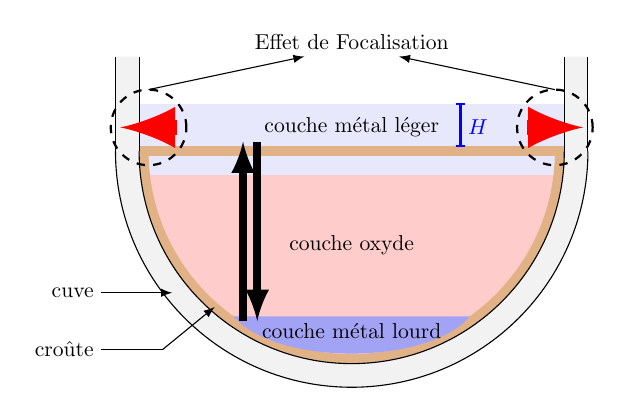
\begin{tikzpicture}[scale = 0.6, every node/.style={scale=0.6}]
        
    
    %cuve
    \fill[gray!10] (0,2) -- (0,0)  arc (180:360:5) -- (10,2) -- (9.5,2) -- (9.5,0) arc (360:180:4.5) -- (0.5,2) -- cycle;
    
    %couche+croute
    \fill[red!20]  (0.5,0) arc (180:360:4.5) -- cycle;
    \fill[blue!80!gray!10](0.5,0) rectangle (9.5, 1);
    \fill[blue!80!gray!10](0.5,0) rectangle (9.5, -0.5);	
    \fill[brown!80!orange!60] (0.5,0) arc (180:360:4.5) -- (9.3,0) arc (360:180:4.3) -- cycle;
    \fill[brown!80!orange!60](0.5,-0.1) rectangle (9.5,0.1);
    
    \fill[blue!80!gray!40]  (2.5,-3.5)  ..controls +(0.9,-1.05)and+(-0.9,-1.05)  .. (7.5,-3.5) -- cycle ;
    
    
    %cuve
    \draw (0,0) arc (180:360:5);
    \draw (0.5,0) arc (180:360:4.5);
    \draw (0,0) -- (0,2);
    \draw (0.5,0) -- (0.5,2);
    \draw (10,0) -- (10,2);
    \draw (9.5,0) -- (9.5,2);
    
    \draw (5,0.5) node[ scale=1.3]{couche métal léger};
    \draw (5,-2) node[ scale=1.3]{couche oxyde};
    \draw (5,-3.8) node[ scale=1.3]{couche métal lourd};
    
    \draw[->,>=latex, red, line width = 2mm] (1.3, 0.5) to (0.1, 0.5);
    \draw[->,>=latex, red, line width = 2mm] (8.7, 0.5) to (9.9, 0.5);
    
    %FE
    \draw[black, dashed, thick] (0.7,0.5) circle (0.8);
    \draw[black, dashed, thick] (9.3,0.5) circle (0.8);
    \draw[->,>=latex] (0.7, 1.3) to (4, 2);
    \draw[->,>=latex] (9.3, 1.3) to (6, 2);
    \draw (5,2.3) node[ scale=1.3]{Effet de Focalisation};
    
    %cuve
    \draw[->,>=latex] (-0.3, -3) to (1.2, -3);
    \draw (-0.3, -3) node[ scale=1.3, left]{cuve};
    
    %croute
    
    \draw[->,>=latex] (1, -4.2) to (2.1, -3.3);
    \draw (1, -4.2) -- (-0.3, -4.2);
    \draw (-0.3, -4.2) node[ scale=1.3, left]{croûte};
    
    %echange
    \draw[->,>=latex,line width = 1mm] (3, 0.2) to (3., -3.6);
    \draw[->,>=latex,line width = 1mm](2.7, -3.6) to  (2.7, 0.2);

\draw[blue, very thick] (7.3, 0.1) -- (7.3, 1);
\draw[blue,  thick] (7.2, 0.1) -- (7.4, 0.1);
\draw[blue,  thick] (7.2, 1) -- (7.4, 1);
  \draw (7.3, 0.5) node[ scale=1.3, right, blue]{$H$};

		\end{tikzpicture}

\end{center}
\end{frame}


\begin{frame}
    \frametitle{Interface de fusion/solidification : la condition de Stefan}
    \footnotesize
    \begin{columns}[c]
        \begin{column}{0.4\textwidth}
		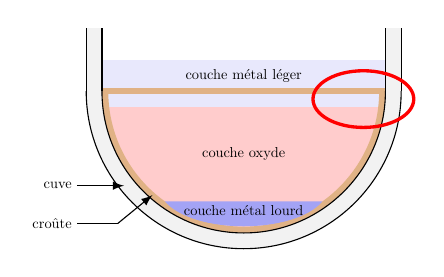
\begin{tikzpicture}[scale = 0.4, every node/.style={scale=0.4}]
        
    
    %cuve
    \fill[gray!10] (0,2) -- (0,0)  arc (180:360:5) -- (10,2) -- (9.5,2) -- (9.5,0) arc (360:180:4.5) -- (0.5,2) -- cycle;
    
    %couche+croute
    \fill[red!20]  (0.5,0) arc (180:360:4.5) -- cycle;
    \fill[blue!80!gray!10](0.5,0) rectangle (9.5, 1);
    \fill[blue!80!gray!10](0.5,0) rectangle (9.5, -0.5);	
    \fill[brown!80!orange!60] (0.5,0) arc (180:360:4.5) -- (9.3,0) arc (360:180:4.3) -- cycle;
    \fill[brown!80!orange!60](0.5,-0.1) rectangle (9.5,0.1);
    
    \fill[blue!80!gray!40]  (2.5,-3.5)  ..controls +(0.9,-1.05)and+(-0.9,-1.05)  .. (7.5,-3.5) -- cycle ;
    
    
    %cuve
    \draw (0,0) arc (180:360:5);
    \draw (0.5,0) arc (180:360:4.5);
    \draw (0,0) -- (0,2);
    \draw (0.5,0) -- (0.5,2);
    \draw (10,0) -- (10,2);
    \draw (9.5,0) -- (9.5,2);
    
    \draw (5,0.5) node[ scale=1.3]{couche métal léger};
    \draw (5,-2) node[ scale=1.3]{couche oxyde};
    \draw (5,-3.8) node[ scale=1.3]{couche métal lourd};
    
    %\draw[->,>=latex, red, line width = 2mm] (1.3, 0.5) to (0.1, 0.5);
    %\draw[->,>=latex, red, line width = 2mm] (8.7, 0.5) to (9.9, 0.5);
    
    %FE
    %\draw[black, dashed, thick] (0.7,0.5) circle (0.8);
    %\draw[black, dashed, thick] (9.3,0.5) circle (0.8);
    %\draw[->,>=latex] (0.7, 1.3) to (4, 2);
    %\draw[->,>=latex] (9.3, 1.3) to (6, 2);
    %\draw (5,2.3) node[ scale=1.3]{Focusing Effect};
    
    %cuve
    \draw[->,>=latex] (-0.3, -3) to (1.2, -3);
    \draw (-0.3, -3) node[ scale=1.3, left]{cuve};
    
    %croute
    
    \draw[->,>=latex] (1, -4.2) to (2.1, -3.3);
    \draw (1, -4.2) -- (-0.3, -4.2);
    \draw (-0.3, -4.2) node[ scale=1.3, left]{croûte};
    
    %echange
    %\draw[->,>=latex,line width = 1mm] (3, 0.2) to (3., -3.6);
    %\draw[->,>=latex,line width = 1mm](2.7, -3.6) to  (2.7, 0.2);

%\draw[blue, very thick] (7.3, 0.1) -- (7.3, 1);
%\draw[blue,  thick] (7.2, 0.1) -- (7.4, 0.1);
%\draw[blue,  thick] (7.2, 1) -- (7.4, 1);
%  \draw (7.3, 0.5) node[ scale=1.3, right, blue]{$H$};


\draw [red,  very thick](8.8,-0.25) ellipse (1.6 and 0.9);

		\end{tikzpicture} 
        \end{column}
\footnotesize
	\begin{column}{0.6\textwidth}
			\begin{itemize}
				\item  Condition de Stefan \bib{Gupta; Stefan} :
						\begin{align} \label{eq:Stefan_cond}
						\vect{u}^\inte &= u^\inte \, \vect{n}^\Gamma = \Frac{1}{\rho^{\Gamma} \Delta \mathcal{H}^{\Gamma}} (\varphi_l - \varphi_s) \, \vect{n}^\Gamma.
						\end{align}
				\item Avec les flux thermiques :
						\begin{align} \label{eq:heat_flux}
						\varphi_k&=\vect{\varphi}_k\cdot\vect{n}^\Gamma,\\
						\vect{\varphi_k} &= -\lambda_k \, \nabla T_k,
						\end{align}
			\end{itemize}
        \end{column}
\normalsize
	\end{columns}
	
\begin{itemize}
	\item Interface entre deux \textbf{matériaux pures homogènes},
	\item Front de fusion/solidification considéré à l'\textbf{équilibre thermodynamique} $\rightarrow$ solide formé à température de solidification,
	\item  \textbf{Interface raide}   $\rightarrow$ Pas de zone de mélange diffuse.
\end{itemize}

\fbox{\begin{minipage}[]{\textwidth}
\begin{center}
 \textcolor{red}{Problème de \textbf{fusion/solidification}  entre \textbf{un liquide chaud et un solide froid}}.\\
\color{red}Caractère \textbf{hétérogène} des conditions à l'interface.
\end{center}
\end{minipage}}
\end{frame}

\begin{frame}
    \frametitle{Identification des interfaces de fusion / solidification : états d'interface}
    \footnotesize
    \begin{columns}[c]
        \begin{column}{0.4\textwidth}
    \begin{center}
		\begin{tikzpicture}[scale = 0.4, every node/.style={scale=0.6}]
        %aires
\fill[blue!95!gray!10] (-0.5,-0.5) -- (-0.5,12) -- (-0.5,12) ..controls +(0,-0.) and +(-0.5,0.3).. (0,11) -- (0,11) ..controls +(1,-0.6) and +(-0.25,0.75).. (2,10) -- (2,10) ..controls +(1,-3) and +(-1.,0.8).. (5,6) -- (5,6) ..controls +(0.5,-0.4) and +(-0.5,0.5).. (5.5,4.5) -- (5.5,4.5) ..controls +(0.5,-0.5) and +(1.5,0.8).. (4,0.5) -- (4,0.5) ..controls +(-0.375,-0.2) and +(0,0).. (3.5,0) -- (3.5,0) ..controls +(0,0) and +(-0,0.).. (3,-0.5) --cycle;

\fill[orange!95!gray!10] (10, -0.5) -- (10, 12) -- (-0.5,12) ..controls +(0,-0.) and +(-0.5,0.3).. (0,11) -- (0,11) ..controls +(1,-0.6) and +(-0.25,0.75).. (2,10) -- (2,10) ..controls +(1,-3) and +(-1.,0.8).. (5,6) -- (5,6) ..controls +(0.5,-0.4) and +(-0.5,0.5).. (5.5,4.5) -- (5.5,4.5) ..controls +(0.5,-0.5) and +(1.5,0.8).. (4,0.5) -- (4,0.5) ..controls +(-0.375,-0.2) and +(0,0).. (3.5,0) -- (3.5,0) ..controls +(0,0) and +(-0,0.).. (3,-0.5) --cycle;

\fill[pattern color = blue, pattern=vertical lines] (-0.5,12) ..controls +(0,-0.) and +(-0.5,0.3).. (0,11) -- (0,11) ..controls +(1,-0.6) and +(-0.25,0.75).. (2,10) -- (2,10) ..controls +(1,-3) and +(-1.,0.8).. (5,6) -- (5,6) ..controls +(0.5,2)  and +(1,-0.3)..  (1,12) ;

\fill[pattern color = orange, pattern=vertical lines]  (2,-0.5)  ..controls +(-1.5,0.8)and+(-0.5,-0.5)  .. (5.5,4.5) --(5.5,4.5) ..controls +(0.5,-0.5) and +(1.5,0.8).. (4,0.5) -- (4,0.5) ..controls +(-0.375,-0.2) and +(0,0).. (3.5,0) -- (3.5,0) ..controls +(0,0) and +(-0,0.).. (3,-0.5) ;



% Gamma
\draw[very thick,  red] (-0.5,12) ..controls +(0,-0.) and +(-0.5,0.3).. (0,11);
\draw[very thick , red](0,11) ..controls +(1,-0.6) and +(-0.25,0.75).. (2,10);
\draw[very thick , red] (2,10) ..controls +(1,-3) and +(-1.,0.8).. (5,6);
\draw[very thick , brown]  (5,6) ..controls +(0.5,-0.4) and +(-0.5,0.5).. (5.5,4.5);
\draw[very thick , blue]  (5.5,4.5) ..controls +(0.5,-0.5) and +(1.5,0.8).. (4,0.5);
\draw[very thick , blue]  (4,0.5) ..controls +(-0.375,-0.2) and +(0,0).. (3.5,0);
\draw[very thick,  blue] (3.5,0) ..controls +(0,0) and +(-0,0.).. (3,-0.5);

%Gamma Dt
\draw[ thin , red, dashed] (1,12) ..controls +(1,-0.3) and +(0.5,2).. (5,6);
\draw[ thin , blue, dashed]  (5.5,4.5) ..controls +(-0.5,-0.5) and +(-1.5,0.8).. (2,-0.5);

% Fleches
\draw[->,>=latex, black] (7.5, 11) to (2.7, 8.4);
\draw[->,>=latex, black] (7.5, 0.5) to (5.4,2.3);


\draw[->,>=latex, black] (8, 5) to (5.3,5);
%texte
\draw (7.5, 1.5) node[rectangle, draw,  fill=white,below, scale=1.5, align =left]{\textbf{interface en} \\ \textbf{solidification}};
\draw (7.5, 10.) node[rectangle, draw,  fill=white, above, scale=1.5, align =left]{\textbf{interface en} \\ \textbf{fusion}};
\draw (8, 5) node[rectangle, draw,  fill=white,  scale=1.5, align =left]{\textbf{interface en} \\ \textbf{conduction}};

\draw (0.2,0) node[ scale=2]{$\Omega_l$};
\draw (4,11.4) node[ scale=2]{$\Omega_s$};

		\end{tikzpicture}

\end{center}
        \end{column}
\footnotesize
	\begin{column}{0.6\textwidth}
    
    \begin{center}
		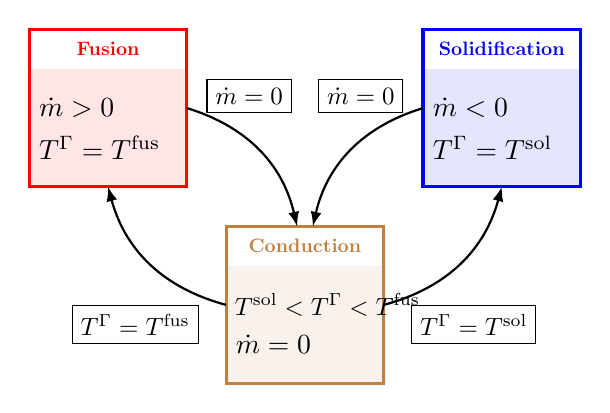
\begin{tikzpicture}[scale = 0.5, every node/.style={scale=0.5}]
        \fill[red!10] (-5,5) rectangle (-1,8);
\fill[blue!10] (5,5) rectangle (9,8);
\fill[brown!10] (0,0) rectangle (4,3);
\draw[red, very thick] (-5,5) rectangle (-1,9);
\draw[brown, very thick] (0,0) rectangle (4,4);
\draw[blue, very thick] (5,5) rectangle (9,9);


\draw (-3, 8.5) node[red , scale=1.4, align =left]{ \textbf{Fusion}};
\draw (7, 8.5) node[blue , scale=1.4, align =left]{ \textbf{Solidification}};
\draw (2, 3.5) node[brown , scale=1.4, align =left]{ \textbf{Conduction}};

\draw (-5, 7.) node[ scale=2,right,align =left]{ $\Dot{m} > 0$};
\draw (-5, 6.) node[ scale=2,right,align =left]{ $T^\Gamma = T^\fus$};

\draw (5, 7.) node[ scale=2,right,align =left]{ $\Dot{m} < 0$};
\draw (5, 6.) node[ scale=2,right,align =left]{ $T^\Gamma = T^\sol$};


\draw (0, 2) node[ scale=1.8,right,align =left]{ $T^\sol<T^\Gamma < T^\fus$ };
\draw (0, 1.) node[ scale=2,right,align =left]{ $ \Dot{m} = 0$};


\draw[->,>=latex, black, thick] (-1., 7) to[bend left] (1.8, 4);
\draw[->,>=latex, black, thick] (5, 7) to[bend right] (2.2, 4);

\draw[->,>=latex, black, thick] (0, 2) to[bend left] (-3, 5);
\draw[->,>=latex, black, thick] (4, 2) to[bend right] (7, 5);

\draw (-0.5, 7.3) node[rectangle, draw,right, scale=1.8]{ $\Dot{m} = 0$};
\draw (4.5, 7.3) node[rectangle, draw,left, scale=1.8]{ $\Dot{m} = 0$};

\draw (-0.7, 1.5) node[rectangle, draw,left, scale=1.8]{ $T^\Gamma = T^\fus$};
\draw (4.7, 1.5) node[rectangle, draw,right, scale=1.8]{ $T^\Gamma = T^\sol$};

		\end{tikzpicture}

\end{center}
        \end{column}
\normalsize
	\end{columns}

\end{frame}


\begin{frame}
    \frametitle{Échelles de modélisation}
    \footnotesize
	\begin{columns}[T]
    	\begin{column}[T]{0.47\textwidth}
    	 \color{cea_rouge}\underline{Échelle de modélisation intégrale :}\color{cea_texte}\\
    	 \begin{itemize}
    	 		\item Modélisation d'une séquence accident grave.
    	 		\item Modèle rapide donc grossier.
    	 		\item Hypothèses de fermetures, corrélations
    	 		\item Utilisation des données provenant des expériences et des modélisations plus fines.
    	 \end{itemize}
    	\end{column}
    	
    	\begin{column}[T]{0.47\textwidth}
    	\color{cea_rouge}\underline{Échelle de modélisation plus fine :}\color{cea_texte}\\
    	  \begin{itemize}
    	 	\item Focalise sur des phénomènes précis.
    	 	\item Utilisation de codes maillés, plus coûteux.
    	 	\item Phénomènes précis déterminés par des expériences ou codes intégraux.
    	 	\item Tend à simuler des situations plus complexes, possible avec l'évolution des moyens de calcul.
    	 \end{itemize}
    	\end{column}
    	\end{columns}
    	\vspace{0.4cm}
    	\begin{center}
    	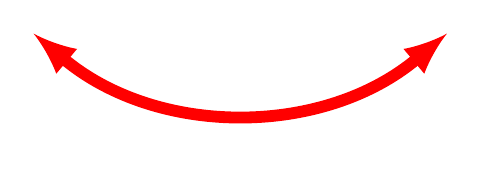
\begin{tikzpicture}[scale = 0.35, every node/.style={scale=0.4}]



		\draw[<->, >=latex, line width = 0.15cm, red] (0,0) to[bend right=40] (15,0);
		

		\end{tikzpicture}
		\end{center}
\end{frame}


\begin{frame}
    \frametitle{Objectifs de la thèse}
    \normalsize
    

        	\begin{ceaalertblock}{Objectifs de la thèse :}
        	
        	Proposer des outils numériques à différents niveaux de modélisation pour suivre ces interfaces de front de fusion/solidification.
        	\begin{itemize}
        		\item Développer des \textbf{modèles et méthodes numériques adaptés} au suivi de ce type particulier d'interface. 
        		\item \textbf{Capacité des méthodes et modèles à évoluer} pour prendre en compte des fermetures thermodynamiques plus complexes.
        		\item \textbf{Implémenter} ces méthodes dans des codes de simulations dédiés.
        		\item \textbf{Valider} ces méthodes sur des cas tests.
        		\item Utiliser ces méthodes dans un \textbf{cadre plus complexe} se rapprochant des problématiques accidents graves. 
        	\end{itemize}
        	\end{ceaalertblock}
\end{frame}
\section*{Sommaire}
%\Titre{Sommaire}
\begin{frame}
\frametitle{Sommaire}
\footnotesize
  \tableofcontents
\end{frame}

\section{Modélisation idéalisée du problème}
\begin{frame}
    \frametitle{Équations considérées}
    \footnotesize

\begin{columns}[T]
    \begin{column}[T]{0.45\textwidth}
    \begin{center}
    \color{cea_rouge}\underline{Pour le solide (équation de la chaleur) :}\color{cea_texte}
    \begin{align*}
    	\rho C_p \frac{\partial T}{\partial t}  &=\nabla\cdot\left(\lambda \nabla T\right) + f,
    \end{align*}
        \end{center}
    \end{column}
    
    
    \begin{column}[T]{0.55\textwidth}
    \begin{center}
\color{cea_rouge}\underline{Pour le liquide (chaleur + Navier-Stokes) :} \color{cea_texte}
\begin{align*}
\nabla. \vect{u} &= 0,\\
\frac{ \partial \vect{u}}{\partial t} + \vect{u}.\nabla \vect{u} &= \frac{-1}{\rho} \nabla p + \nu \Delta \vect{u} - \mathcal{B}(T-T^{\text{ref}}) \vect{g} ,\\
\rho C_p (\frac{\partial T}{\partial t} + \vect{u} \cdot \nabla T ) &= \nabla\cdot\left(\lambda \nabla T\right) + f,
\end{align*}
    \end{center}
\end{column}
\end{columns}
\hspace{-1.8cm}
\begin{center}
\color{cea_rouge}\underline{Pour l'interface liquide-solide (condition de Stefan) :}\color{cea_texte}
\begin{align*}
	\vect{u}^\Gamma &= u \, \vect{n}^\Gamma = \frac{1}{\rho^{\Gamma} \Delta \mathcal{H}^{\Gamma}} (\varphi_l - \varphi_s) \, \vect{n}^\Gamma,
\end{align*}
où $\Gamma$ sert à \textbf{différencier les paramètres} de fusion et de solidification,\\
\vspace{0.3cm}
qui seront \textbf{déduits des  compositions} des liquides et des solides.
\end{center}
\vspace{0.1cm}
	\fbox{\begin{minipage}[]{\textwidth}
	\center\textcolor{red}{+ Fermetures à l'interface à définir}
	\end{minipage}}
\end{frame}

\begin{frame}
\frametitle{Fermetures thermiques à l'interface}
\footnotesize


\begin{center}
		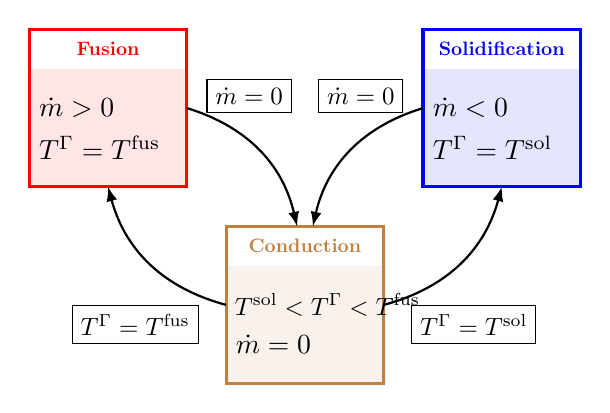
\begin{tikzpicture}[scale = 0.5, every node/.style={scale=0.5}]
			\fill[red!10] (-5,5) rectangle (-1,8);
\fill[blue!10] (5,5) rectangle (9,8);
\fill[brown!10] (0,0) rectangle (4,3);
\draw[red, very thick] (-5,5) rectangle (-1,9);
\draw[brown, very thick] (0,0) rectangle (4,4);
\draw[blue, very thick] (5,5) rectangle (9,9);


\draw (-3, 8.5) node[red , scale=1.4, align =left]{ \textbf{Fusion}};
\draw (7, 8.5) node[blue , scale=1.4, align =left]{ \textbf{Solidification}};
\draw (2, 3.5) node[brown , scale=1.4, align =left]{ \textbf{Conduction}};

\draw (-5, 7.) node[ scale=2,right,align =left]{ $\Dot{m} > 0$};
\draw (-5, 6.) node[ scale=2,right,align =left]{ $T^\Gamma = T^\fus$};

\draw (5, 7.) node[ scale=2,right,align =left]{ $\Dot{m} < 0$};
\draw (5, 6.) node[ scale=2,right,align =left]{ $T^\Gamma = T^\sol$};


\draw (0, 2) node[ scale=1.8,right,align =left]{ $T^\sol<T^\Gamma < T^\fus$ };
\draw (0, 1.) node[ scale=2,right,align =left]{ $ \Dot{m} = 0$};


\draw[->,>=latex, black, thick] (-1., 7) to[bend left] (1.8, 4);
\draw[->,>=latex, black, thick] (5, 7) to[bend right] (2.2, 4);

\draw[->,>=latex, black, thick] (0, 2) to[bend left] (-3, 5);
\draw[->,>=latex, black, thick] (4, 2) to[bend right] (7, 5);

\draw (-0.5, 7.3) node[rectangle, draw,right, scale=1.8]{ $\Dot{m} = 0$};
\draw (4.5, 7.3) node[rectangle, draw,left, scale=1.8]{ $\Dot{m} = 0$};

\draw (-0.7, 1.5) node[rectangle, draw,left, scale=1.8]{ $T^\Gamma = T^\fus$};
\draw (4.7, 1.5) node[rectangle, draw,right, scale=1.8]{ $T^\Gamma = T^\sol$};

		\end{tikzpicture}

\end{center}
\begin{ceablock}{Fermetures à l'interface considérées :}
\begin{align}
	(\mathcal{F}) &:\left\{ \begin{array}{ll}
T=T^\sol,  \; &\text{ si } \Dot{m} \leq 0, \\
\vect{\varphi}_s \cdot \norm^\inte= \vect{\varphi}_l \cdot \norm^\inte,  \; &\text{ si } T^\sol < T^\inte < T^\fus,\\
T=T^\fus,   \; &\text{ si } \Dot{m}>0.
 \end{array}\right.
\end{align}
\end{ceablock}
\end{frame}

%--------------------------------------------------------------------------
%==========================================================================
%--------------------------------------------------------------------------

\Intercalaire{Simulation d'une interface en deux dimensions par couplage de modèles 0D et 2D dans un code intégral}
\section{Simulation d'une interface en deux dimensions par couplage de modèles 0D et 2D dans un code intégral}
\subsection{Environnement de travail}
\begin{frame}
    \frametitle{Présentation du code \procor{} :}
    \scriptsize
    %!! Code intégral, couplage de modèle, 0D, analyse de sensibilité, contrainte imposées par AG, partionnement.
      \begin{ceablock}{Contraintes imposées par le contexte AG}
		\begin{itemize}
			\item \textbf{Multi-physique et multi-échelle} : neutronique, thermique, thermohydraulique, mécanique, chimique ... 
			\item Peu de données.
		\end{itemize}
    \end{ceablock}
    \begin{ceablock}{Conséquences sur \procor{} :}
		\begin{itemize}
			\item Études statistiques de sensibilité : implémentation de \textbf{modèles rapides} (modèles 0D)
			\item Architecture spécifique, pensée pour le couplage de modèles \bib{Viot et al. 2018}. Paradigme de \textbf{partitionnement de modèle}.
		\end{itemize}
    \end{ceablock}
    \begin{center}
    	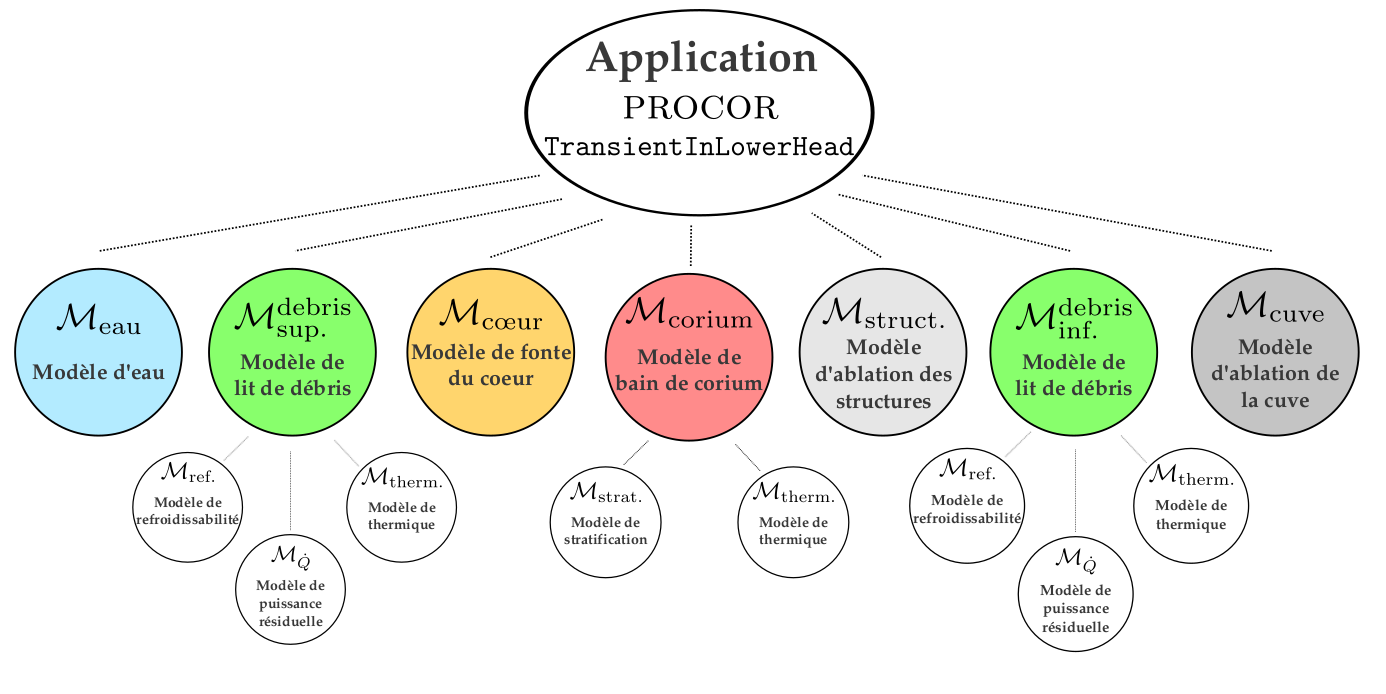
\includegraphics[width=0.7\textwidth]{Figures/applicationProcor.png}
    \end{center}
\end{frame}



\begin{frame}
    \frametitle{Modèle d'interface 0D}
   \footnotesize
   \underline{Première hypothèse} : \textbf{géométrie rectangulaire "multi-1D"}.\\
   \vspace{0.3cm}

 \color{cea_rouge} \underline{Condition d'interface 0D :}  \color{cea_texte} $$ \dot{m} =  \frac{mes(\Gamma)}{\Delta H_{fus}} (\overline{\varphi}_l^{ls}(t) -\overline{\varphi}_s^{ls}(t))$$
\color{cea_rouge} \underline{Équation 0D du solide} : \color{cea_texte} $$ \frac{\partial m_s}{\partial t} = -\dot{m} \, \, \textbf{ et }  \, \, C_s (m_s \frac{d\overline{T_s}}{dt} + \dot{m} (T_{\Gamma} - \overline{T_s} )) = -\overline{\varphi}^i_s \times mes(\delta \Omega_s \setminus \Gamma)    + \overline{\varphi}^{ls, i}_s \times mes(\Gamma) $$

\color{cea_texte!70}	Ce sont principalement des équations bilans. Deux variables suivies : la température moyenne du solide $\overline{T_s}$ et la masse du solide $m_s$.\color{cea_texte}
%These are mainly balanced equation. They follow two variables : the mean temperature of the solid and the mass of the solid.
%Two hypotesis are needed to close the model : one on the \textbf{geometry of the solid} and another one on the \textbf{temperature profil}
\begin{columns}[c]
	\begin{column}{0.55\textwidth}
	%\underline{Première hypothèse} : \textbf{Géométrie rectangulaire "multi-1D".\footnotemark[2]} \\% Solid is considered rectangular, and mass and thermal exchange are only autorized through right and left border. \\
	\underline{Deuxième hypothèse} : \textbf{profil de température quadratique \bib{Le Tellier et al.}}.\\
	\color{cea_texte!70} $\Rightarrow$ Sol. stationnaire de l'équation de la chaleur 1D. \color{cea_texte}
	% profil is considered. Chosen after 	a study on many other possibilities (see ??). This profil corresponds to a stationnary solution.
	\vspace{0.5cm}
	\fbox{\begin{minipage}[]{\textwidth}
	\center\textcolor{red}{On va lever ces deux hypothèses.}
	\end{minipage}}
	\end{column}
    \begin{column}{0.45\textwidth}
	\begin{center} 
	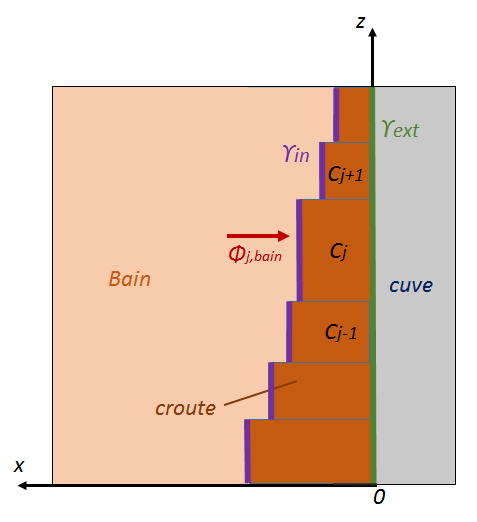
\includegraphics[width=0.62\textwidth]{Figures/modele_croute_0D.png}
			
		\end{center}
		\end{column}
\end{columns}
%\footnotetext[2]{\tiny Le Tellier, R., Skrzypek, E., Saas, L., 2017. On the treatment of plane fusion front in lumped parameter thermal models with convection.}
\end{frame}

\subsection{Présentation du nouveau modèle}
\begin{frame}
    \frametitle{Modèle d'interface 2D}
	\footnotesize
	\begin{ceablock}{Équations considérées :}
		\begin{eqnarray*}  \label{eq:IdealCrust_Temp}
			\rho_s C_s \frac{\partial T_s}{\partial t}  &=& \lambda_s \Delta T_s  \text{ \, (Modèle du solide) }\\
			\vect{u} &=&\frac{1}{\rho^{\Gamma} \Delta \mathcal{H}^{\Gamma}} (\vect{\varphi}_l - \vect{\varphi}_s) \cdot  \vect{n} \text{ \, ( Modèle d'interface ) }\\
			&+&\text{ couplage avec les modèles 0D }
		\end{eqnarray*}
	\end{ceablock}
	
	
	\begin{columns}[c]
	\begin{column}{0.5\textwidth}
	\begin{ceablock}{Couplage des sous-modèles:}
	%%%%%%%%%%%%
		\begin{tikzpicture}[scale = 0.35, every node/.style={scale=0.4}]

		%%def des systemes
		\node[draw, ellipse, fill=gray!10, text centered,text width = 3.5cm,  minimum width = 5cm, minimum height = 4cm] (corium) at (0,1.0) {\Large{Autres modèles}};

		\node[draw, ellipse, fill=gray!10, text centered,text width = 3.5cm,  minimum width = 5cm, minimum height = 4cm] (croute) at (10,0.0) {\Large{Modèle du solide}};

		\node[draw, ellipse, fill=gray!10, text centered,text width = 3.5cm,  minimum width = 5cm, minimum height = 4cm] (stefan) at (6,7.0) {\Large{Modèle de l'interface}};


		%% mise en place des relations


		\draw[->, >=latex, line width = 0.05cm] (corium) to[bend right =15 ]  (croute);
		\node[draw, fill = white] at  (5,-0.5){\large{$\varphi_l$}};

		\draw[->, >=latex, line width = 0.05cm] (croute) to[bend right=15]  (corium);
		\node[draw, fill = white] at  (5,1.5){\large{$\varphi_s$}};

		\draw[->, >=latex, line width = 0.05cm] (croute) to[bend right=15]  (stefan);
		\node[draw, fill = white] at  (9.0,3.5){\large{$\varphi_s$}};

		\draw[->, >=latex, line width = 0.05cm] (stefan) to[bend right=15]  (croute);
		\node[draw, fill = white] at  (7,3.5){\large{$u$}};

		\draw[->, >=latex, line width = 0.05cm] (corium) to[bend right=15]  (stefan);
		\node[draw, fill = white] at  (3.6,3.4){\large{$\varphi_l$}};

		\draw[->, >=latex, line width = 0.05cm] (stefan) to[bend right=15]  (corium);
		\node[draw, fill = white] at  (2.3,4.5){\large{$u$}};

		\end{tikzpicture}
	%%%%%%%%%%%%
		\end{ceablock}
	\end{column}
	\begin{column}{0.5\textwidth}
\scriptsize
\begin{center}
    

		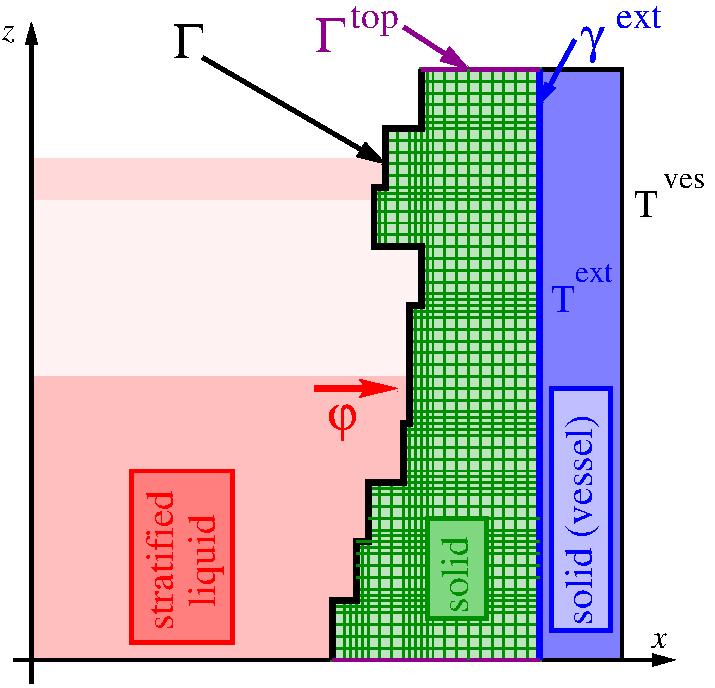
\includegraphics[width=0.65\textwidth]{Figures/ideal2D_sketch.pdf}
\end{center}
    
	\end{column}
	\end{columns}



\end{frame}

\begin{frame}
    \frametitle{Résolution du modèle d'interface 2D}
    \footnotesize
	\begin{ceablock}{Discrétisation et déplacement de l'interface :}
	\begin{columns}[c]
	\begin{column}{0.7\textwidth}
	\begin{itemize}
		\item Interface maillée par des \textbf{segments verticaux et horizontaux}.\\
        \item Association à chaque segment des paramètres ($T_{fus}$, $\Delta \mathcal{H}^{fus}$, ...).\\
        \item Déplacements verticaux et horizontaux.\\
        \item Déplacements 2D, par \textbf{splitting directionnel}.\\
        \item \textbf{Reconstruction du maillage} de l'interface à chaque pas de temps.\\
        \item Donc projection de certains paramètres (température et état du segment) d'une interface à l'autre.
	\end{itemize}
	
	\end{column}
	\begin{column}{0.3\textwidth}
	\begin{center}
		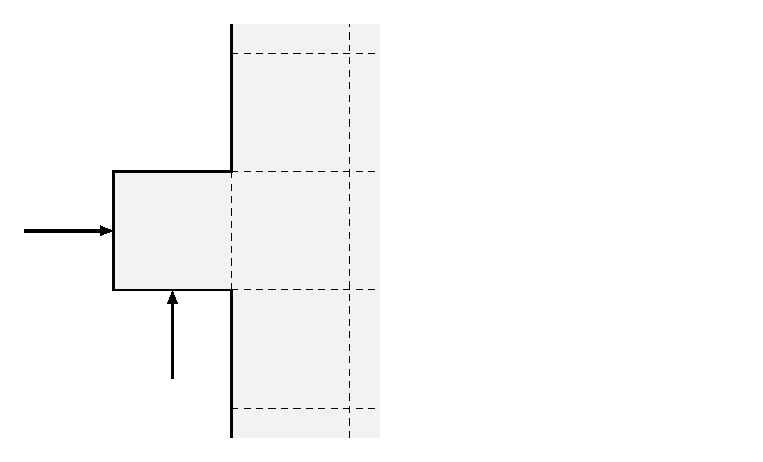
\includegraphics[width=1.55\textwidth]{Figures/interface.pdf}
	\end{center}

	\end{column}

	\end{columns}
	\center \fbox{\color{red}{$\bm{\varphi_l}$ est obtenu par le modèle liquide et $\bm{\varphi_s}$  par le modèle solide.}}
		\end{ceablock}
	\end{frame}
	
\begin{frame}
    \frametitle{Résolution du modèle solide}
    \footnotesize


\begin{columns}[c]
	\begin{column}{0.6\textwidth}
	\begin{ceablock}{Résolution du solide par éléments finis mixtes :}
\begin{enumerate}
			\item \textbf{Remaillage}: adaptation du maillage à la nouvelle interface.
			\item \textbf{Projection}: de la température sur le nouveau maillage (utilisation des fonctions éléments finis).
			\item \textbf{Résolution}: de l'équation de la chaleur avec l'élément mixte de Raviart-Thomas. \bib{Project Fenics}
		\end{enumerate}
\center $\Rightarrow$ \textbf{Identification} directe des flux thermiques à l'interface.
		\end{ceablock}
	\end{column}
	\begin{column}{0.5\textwidth}
	\center
		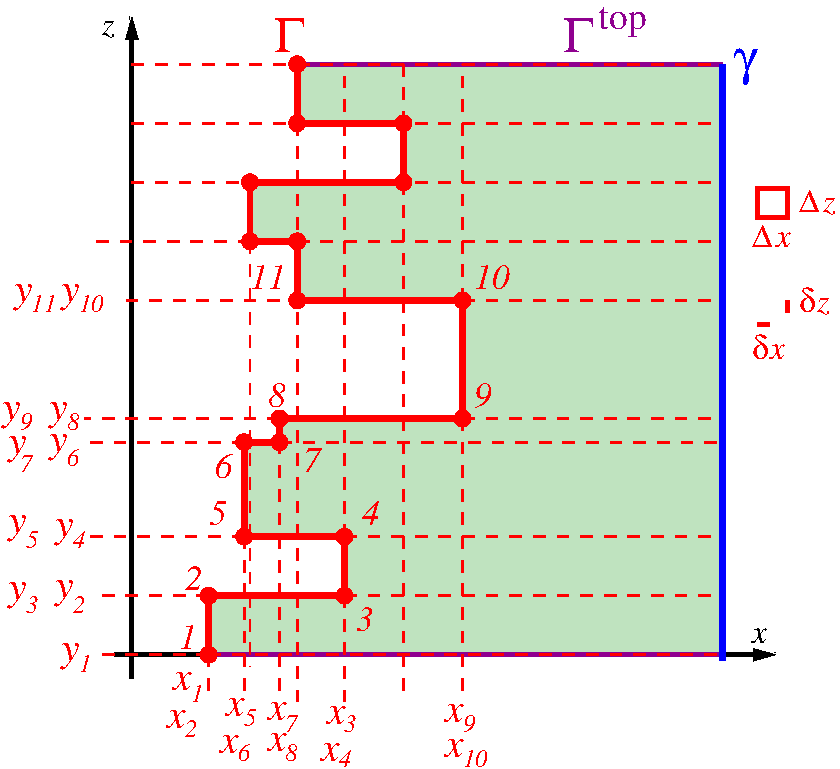
\includegraphics[width=0.65\textwidth]{Figures/crust_mesh.pdf}\\
		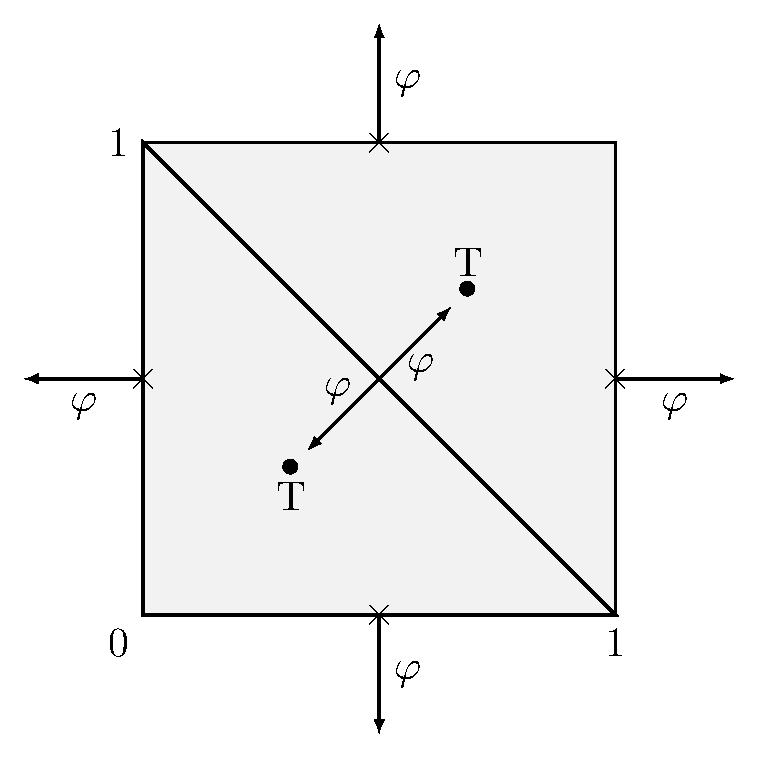
\includegraphics[width=0.65\textwidth]{Figures/elementFiniMixte2.pdf}

		
			\end{column}

	\end{columns}

\end{frame}

%\begin{frame}
%\frametitle{Algorithme final}
%\footnotesize
%	\begin{ceablock}{Algorithme final, en utilisant un schéma semi-explicite:}	
%        \begin{enumerate}
%            \item Résolution de l'équation de la chaleur par méthode élément finis
%            $$\left( (\Omega_s)_h^n, (T_j^{n})_{j=1, \ldots, N_j^n}, \, \text{BCs}, \right) \longrightarrow \quad  ( T_j^{n+1}, (\vec{\varphi}_j^{n+1})_{j=1, \ldots, N_j^n} )$$
%            \item Déplacement de l'interface
%            $$\left( \Gamma^{{n}}, 
%((\lambda\nabla T)_j^{n+1})_{j=1, \ldots, N_j^n}
%(\vec{\varphi}_j)_{j=1, \ldots, N_j^n}, \, \text{BCs}, \right) \longrightarrow\quad   \Gamma^{{n+1}} $$
 %           \item Remaillage du solide avec la nouvelle interface
%            $$\left( \Omega_s^n, (\Omega_s)_h^n, \Gamma^{{n+1}} \right) \longrightarrow \quad   \left( \Omega_s^{n+1}, (\Omega_s)_h^{n+1} \right)$$
%            \item Projection de l'ancienne température sur le nouveau domaine
%            $$\left( (\Omega_s)_h^{n+1}, (\Omega_s)_h^{n}, (T_j^{n+1})_{j=1, \ldots, N_j^n} \right) \longrightarrow \quad   ( T_k^{n+1} )_{k=1, \ldots, N_k^{n+1}}$$
%        \end{enumerate}
%    \end{ceablock}
%\end{frame}

\subsection{Résultats}
\begin{frame}
    \frametitle{Résultats : validation cas test de Stefan, angle 2D}
    \scriptsize
	\color{cea_rouge}\underline{Problème de Stefan 1D :} \color{cea_texte}
	\begin{center}

		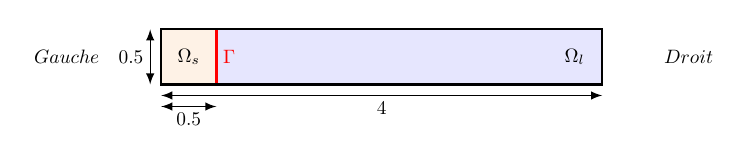
\begin{tikzpicture}[scale = 0.7, every node/.style={scale=0.7}]
			
\fill[orange!95!gray!10] (0,0) rectangle (1,1);
\fill[blue!95!gray!10] (1,0) rectangle (8,1);
\draw[red, very thick] (1,0) -- (1,1);

\draw (0.5, 0.5) node[ scale=1.]{$\Omega_s$};
\draw (7.5, 0.5) node[scale=1]{$\Omega_l$};


\draw[  thick] (0, 0.) rectangle(8, 1);

\draw[<->,>=latex] (0, -0.2) to (8, -0.2);
\draw[<->,>=latex] (0, -0.4) to (1, -0.4);
\draw[<->,>=latex] (-0.2, -0.) to (-0.2, 1);

\draw (.5, -0.4) node[scale=1, below]{$0.5$};
\draw (4, -0.2) node[scale=1, below]{$4$};
\draw (-0.2, 0.5) node[scale=1, left]{$0.5$};
\draw (1, 0.5) node[scale=1, right, red]{$\Gamma$};


\draw (-1, 0.5) node[scale=1, left]{$Gauche$};
\draw (9, 0.5) node[scale=1, right]{$Droit$};



		\end{tikzpicture}


	\begin{table}
	\centering
	%    \hspace{-2cm}
	\resizebox{.89\textwidth}{!}{
		\begin{tabular}{c|ccc}
			\hline
			$\Delta t$ & $L_1$ error & $L_2$ error & $L_\infty$ error \\
			\hline
			$1.0$ & $2.87\times 10^{-1}$ & $3.11\times 10^{-1}$& $8.33\times 10^{-1}$\\
			$0.5$ & $9.70\times 10^{-2}$ & $1.04\times 10^{-1}$& $2.92\times 10^{-1}$\\
			$0.3$  & $4.75\times 10^{-2}$ & $4.90\times 10^{-2}$& $1.03\times 10^{-1}$\\
			$0.1$ & $1.18\times 10^{-2}$ & $1.28\times 10^{-2}$& $8.48\times 10^{-2}$\\
			
			\hline
		\end{tabular} 
		\hspace{-0.1cm}
		\begin{tabular}{c|ccc}
			\hline
			$\Delta x$ & $L_1$ error & $L_2$ error & $L_\infty$ error \\
			\hline
			$0.6$  & $1.30\times 10^{-1}$ & $1.31\times 10^{-1}$& $2.00\times 10^{-1}$\\
			$0.3$  & $7.85\times 10^{-2}$ & $7.93\times 10^{-2}$& $1.24\times 10^{-1}$\\
			$0.2$  & $8.89\times 10^{-2}$ & $5.81\times 10^{-2}$& $1.03\times 10^{-1}$\\
			$0.1$  & $4.75\times 10^{-2}$ & $4.90\times 10^{-2}$& $1.03\times 10^{-1}$\\
			$0.05$ & $3.97\times 10^{-2}$ & $4.13\times 10^{-2}$& $9.26\times 10^{-2}$\\
			\hline
	\end{tabular} }
	
\end{table}
\end{center}
\begin{columns}[t]
	\begin{column}{0.39\textwidth}
    \textcolor{cea_rouge}{\underline{Cas test de l'angle 2D \bib{Rathjen et al.} :}}%(Schéma à gauche, résultat à droite)
\begin{center}
        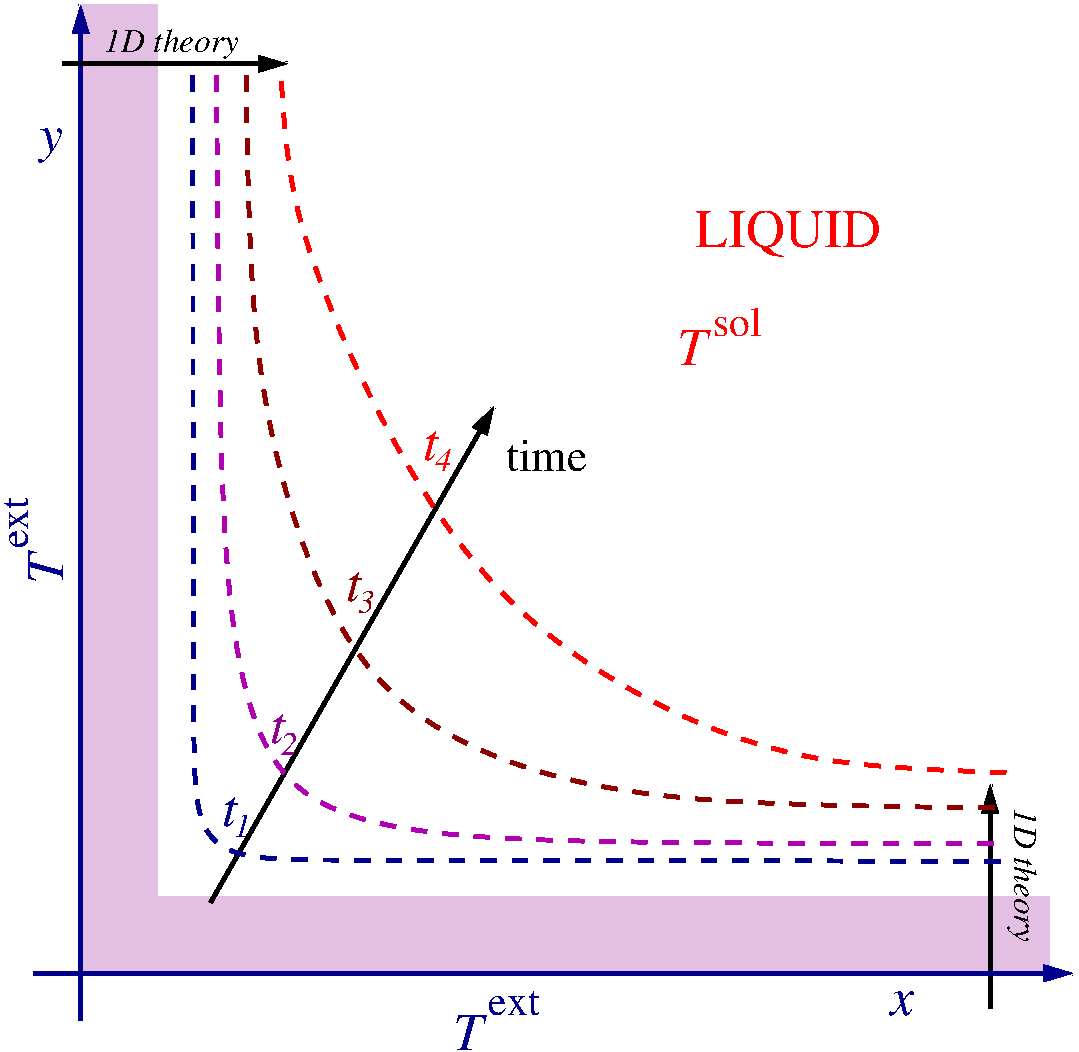
\includegraphics[width=0.60\textwidth]{Figures/2DStefan.pdf}
        \end{center}
        \end{column}
		\begin{column}{0.59\textwidth}
		\begin{center}
		\vspace{-1.2cm}
        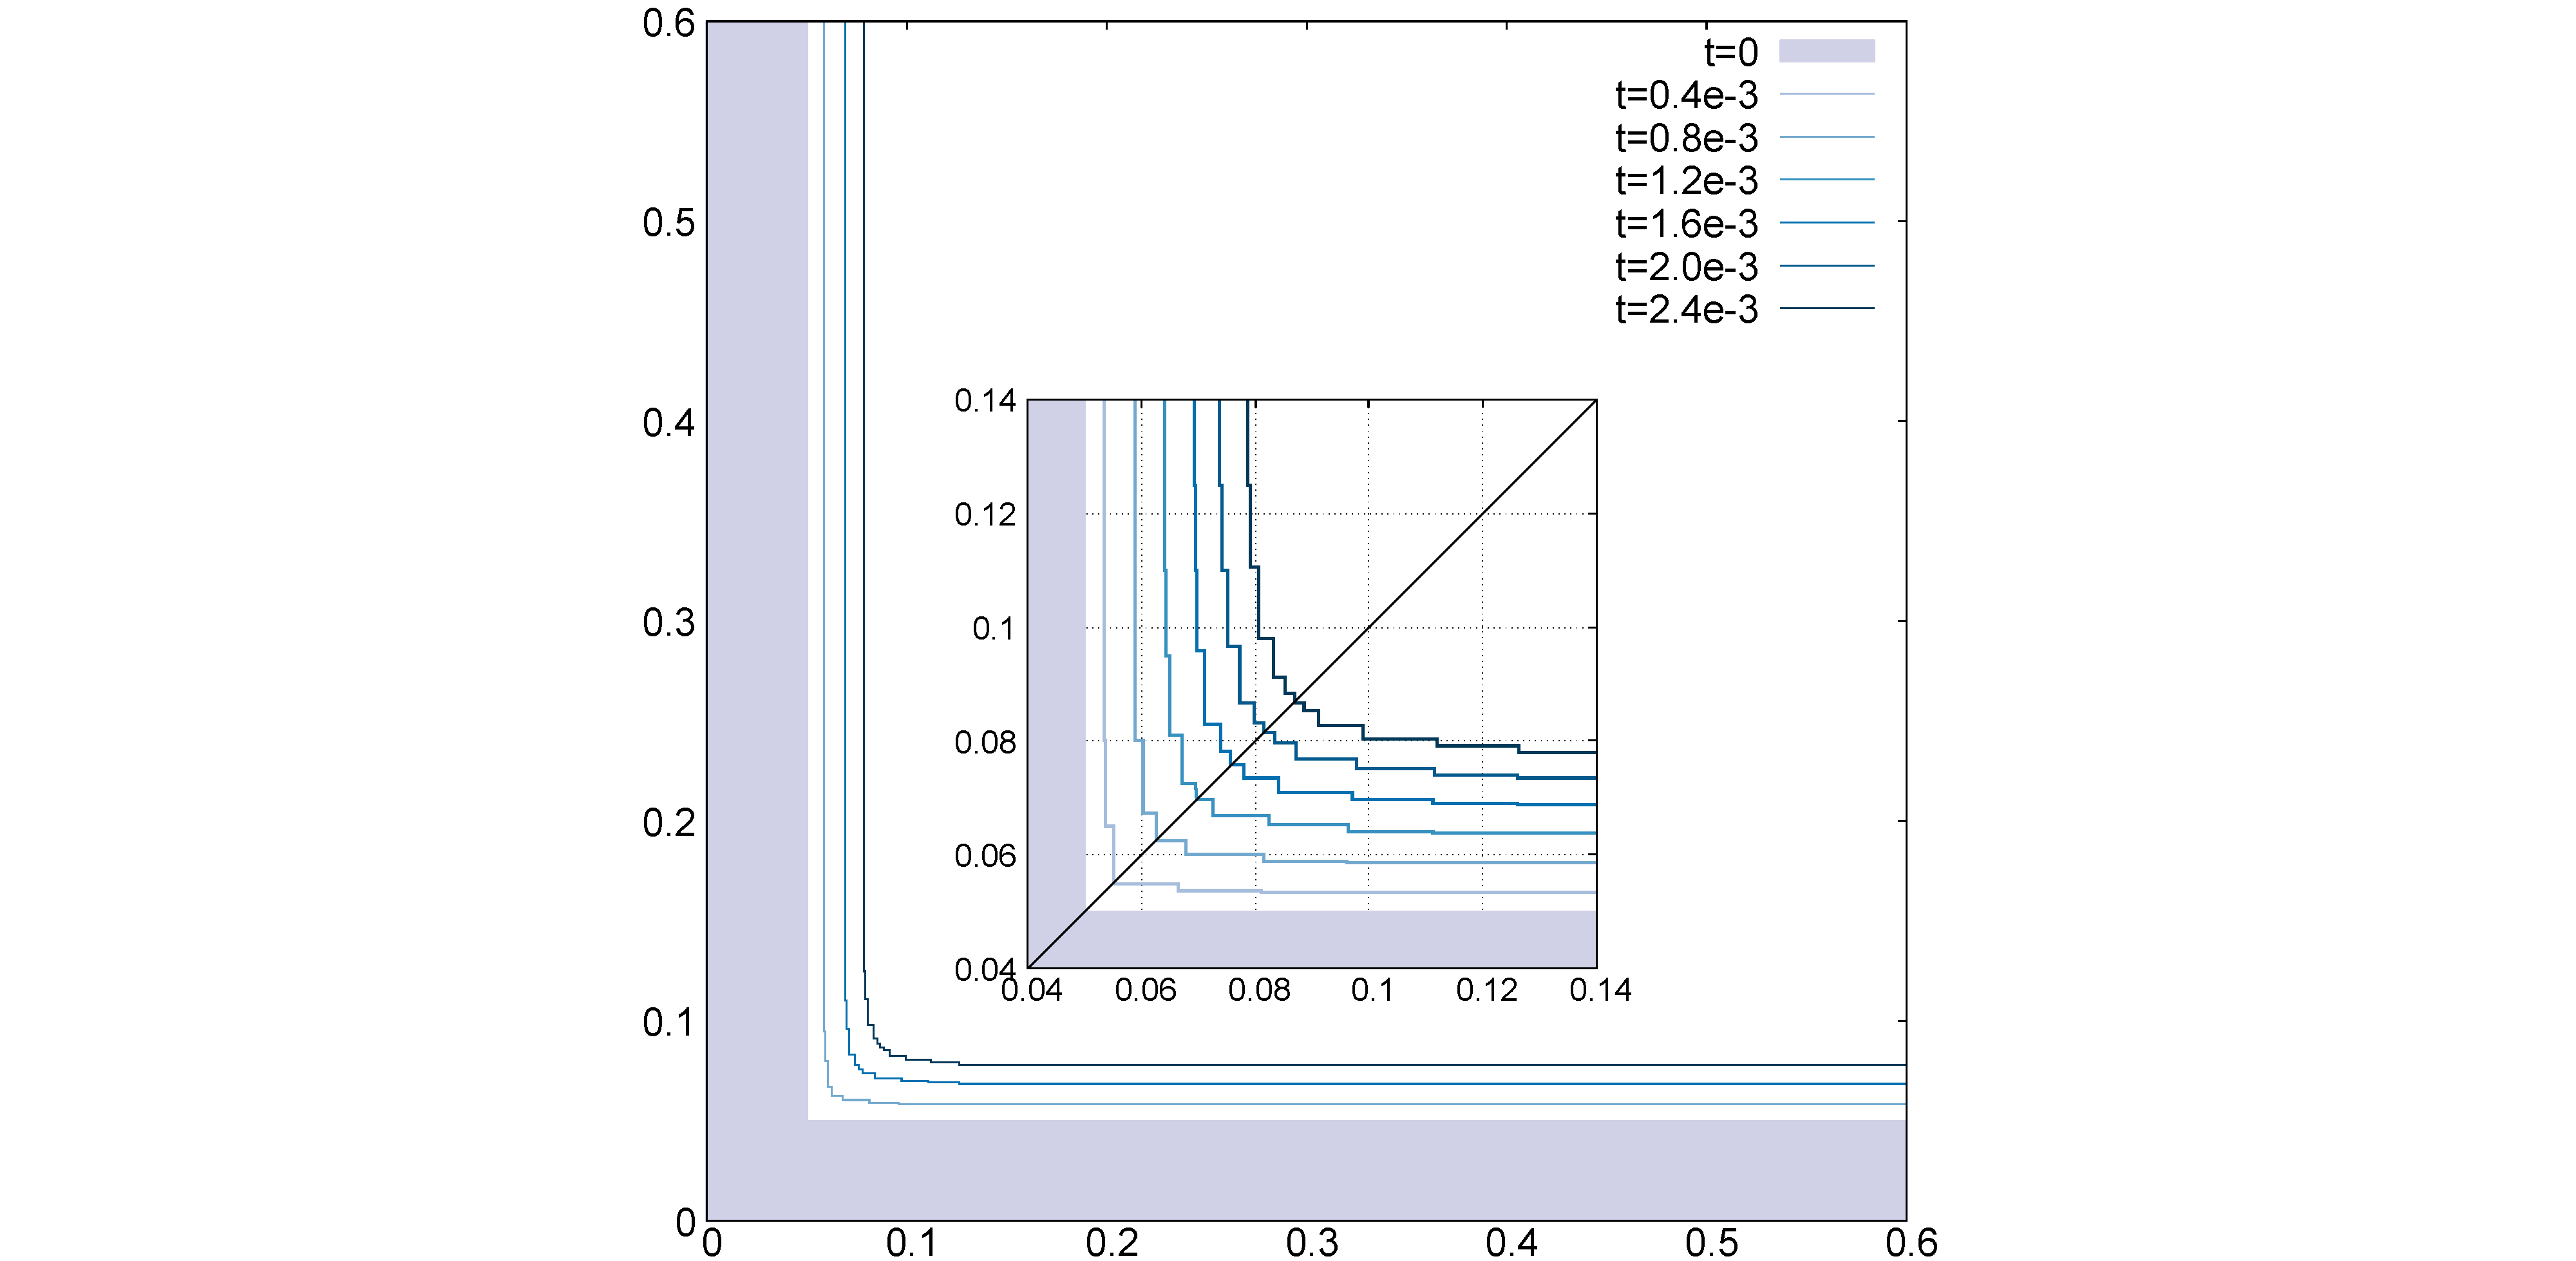
\includegraphics[width=1.2\textwidth]{Figures/Angle2D2_2.pdf}
        \end{center}
        \end{column}
        \end{columns}


\end{frame}

\begin{frame}
    \frametitle{Présentation du cas test de croûte}
 \scriptsize
    \underline{Objectif} : utilisation du modèle 2D dans une simulation plus complexe (+ couplage à d'autres modèles). Simulation de la \textbf{formation de la croûte} pendant une stratégie IVR. Trois étapes \bib{Viot et al. 2020}:
    
    \begin{itemize}
        \item \color{cea_texte!70}Bain de corium tout oxyde $\rightarrow$ Formation d'une croûte tout oxyde.
        \item Ajout d'élément métallique dans le corium liquide $\rightarrow$ Stratification du bain de corium.
        \item Décroissance artificielle de la chaleur résiduelle dans le corium liquide  $\rightarrow$ Solidification massive.\color{cea_texte}
    \end{itemize}
    \begin{center}
    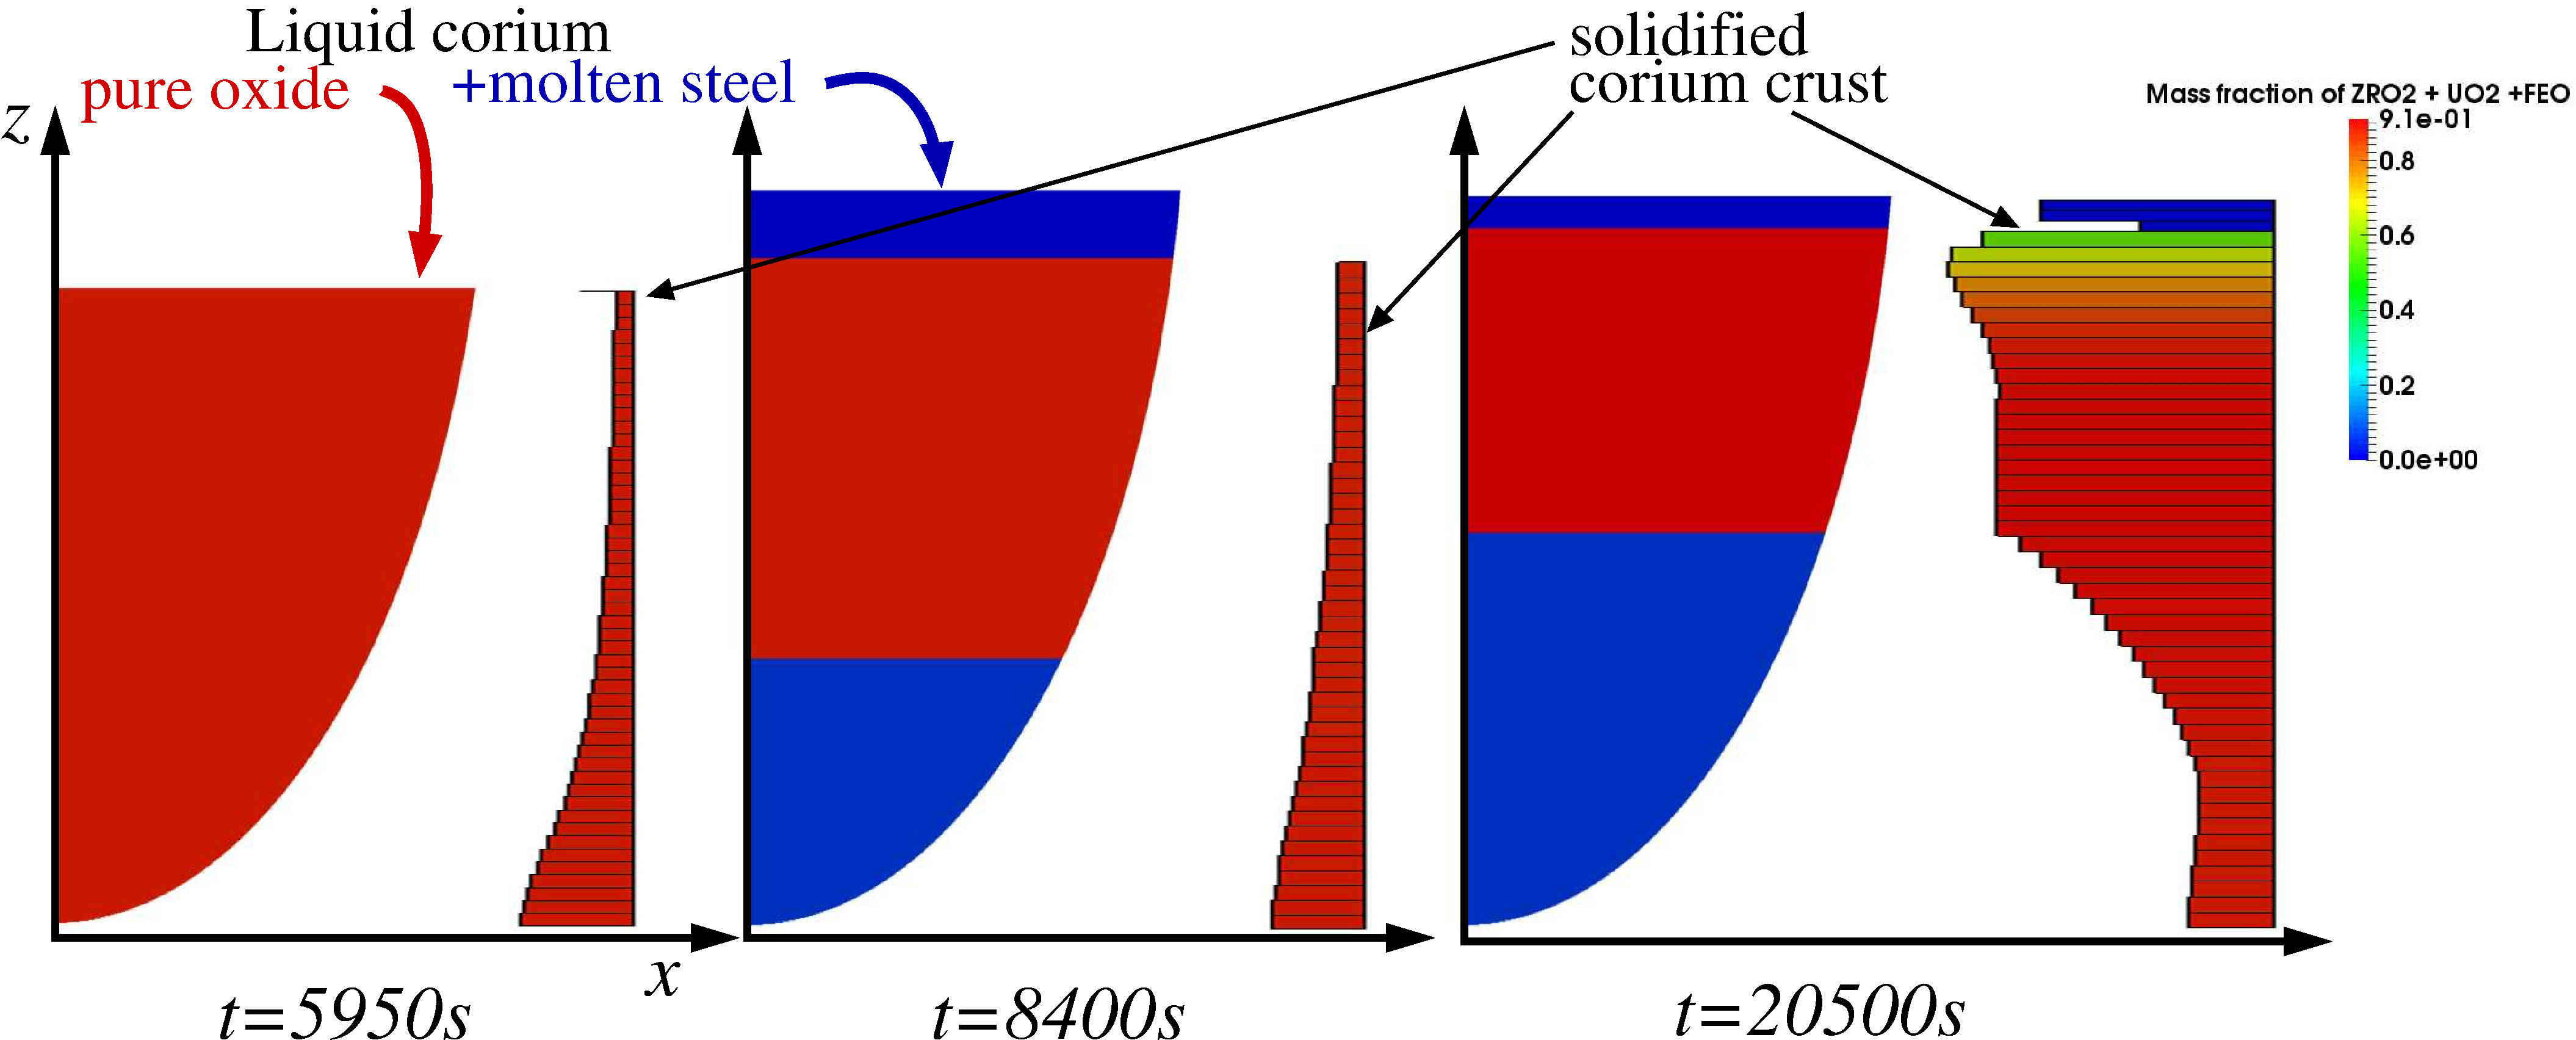
\includegraphics[width=0.95\textwidth]{Figures/industrial_test_sketch.pdf}
    \end{center}
    
        	\begin{ceaalertblock}{Restriction sur le modèle 2D}
        	\tiny
        	En raison du couplage avec les autres modèles 0D, \textbf{les déplacements verticaux de l'interface sont supprimés}.
    	\end{ceaalertblock}
    
\end{frame}


\begin{frame}[t]
    \frametitle{Cas test de formation de la croûte}
	\footnotesize
	
    Plusieurs comparaisons ont été réalisées entre le modèle d'interface 0D et le nouveau modèle d'interface 2D.\\

    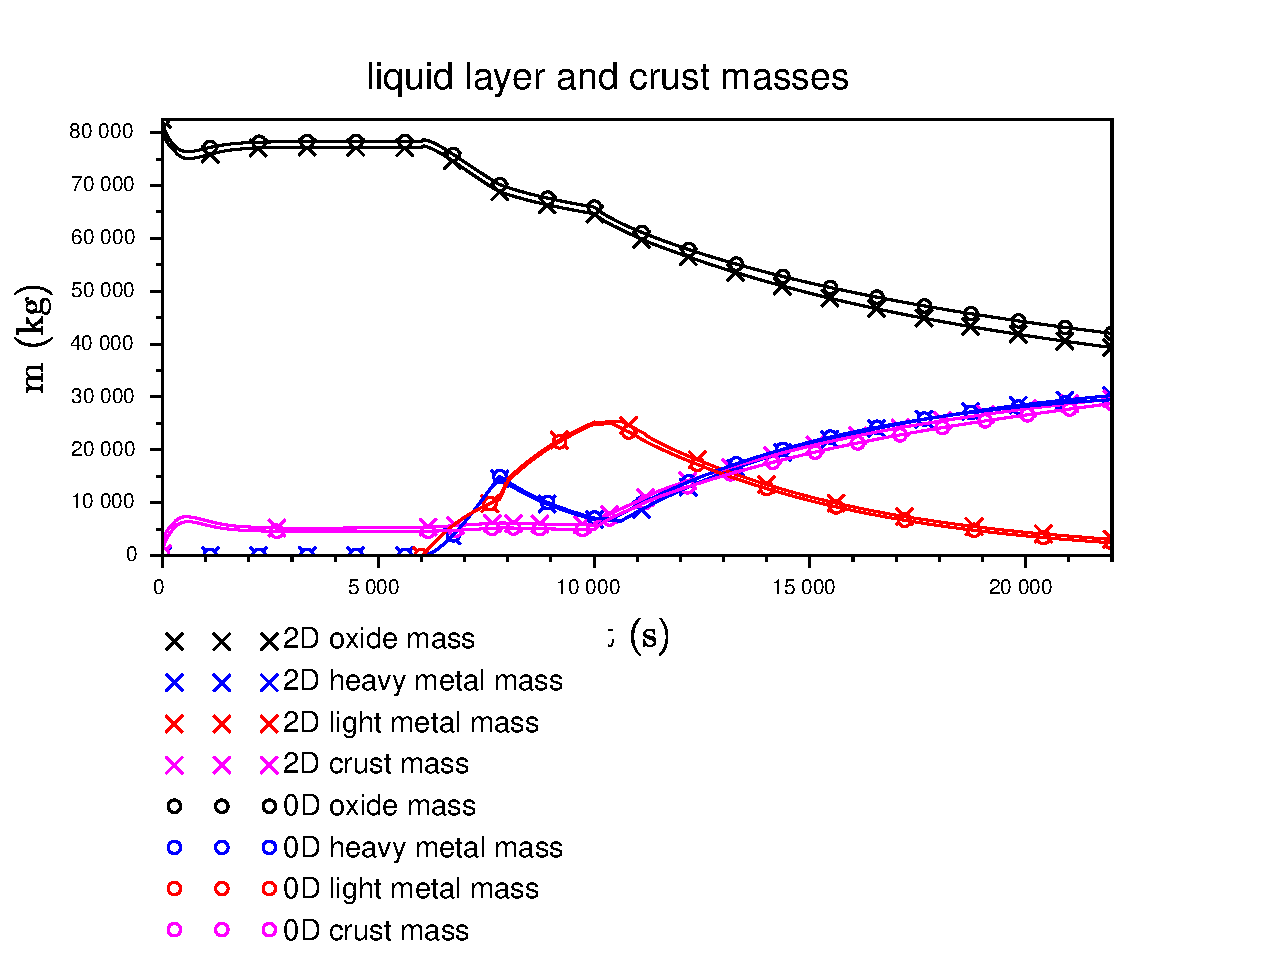
\includegraphics[width=0.47\textwidth]{Figures/IndustrialTestmasses.pdf}
    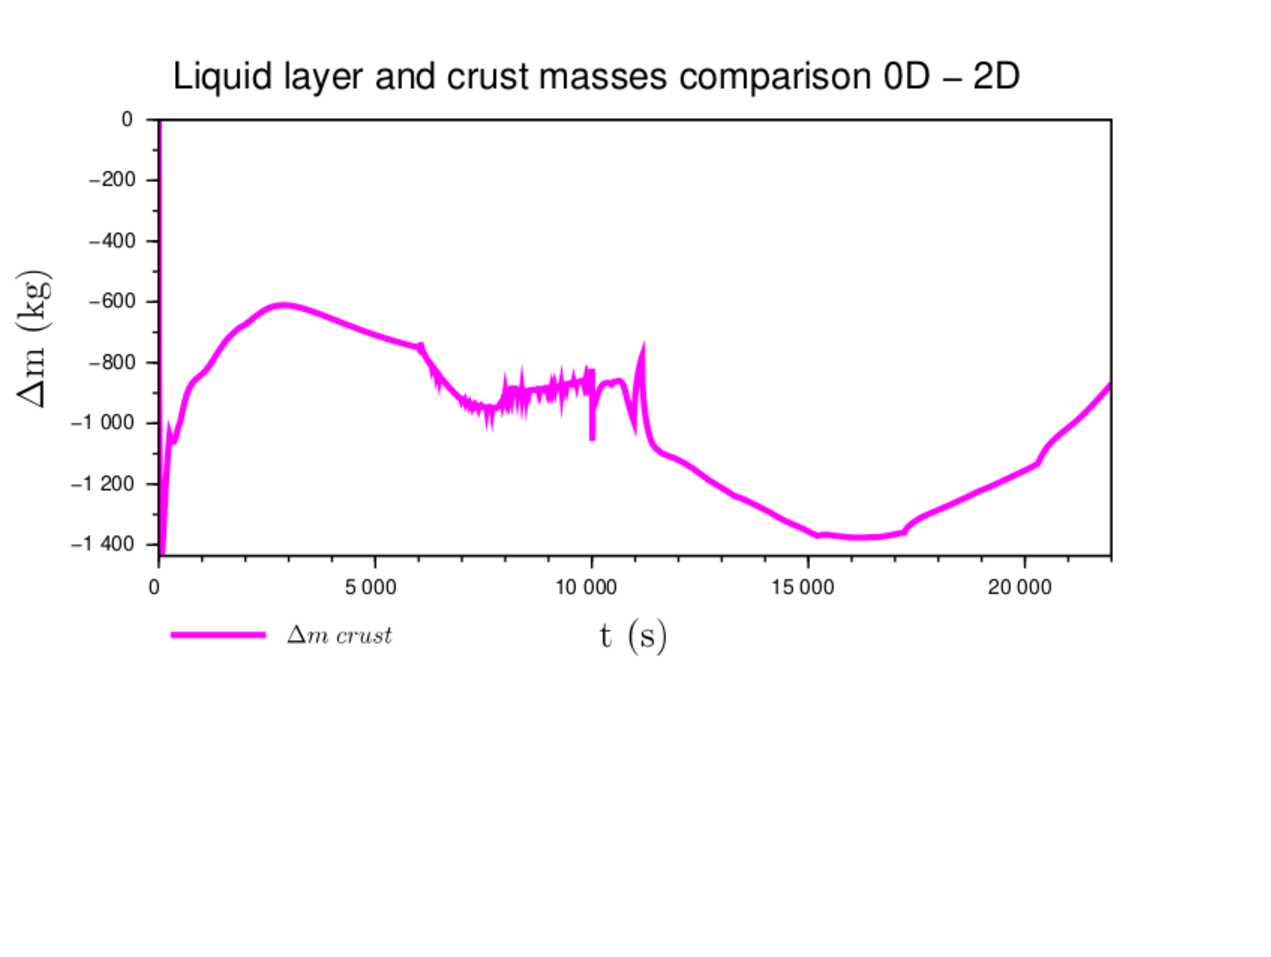
\includegraphics[width=0.47\textwidth]{Figures/IndustrialTestdiffMasses.pdf}

\end{frame}
\begin{frame}[t,noframenumbering]
    \frametitle{Cas test de formation de la croûte}
\footnotesize
    Plusieurs comparaisons ont été réalisées entre le modèle d'interface 0D et le nouveau modèle d'interface 2D.\\
   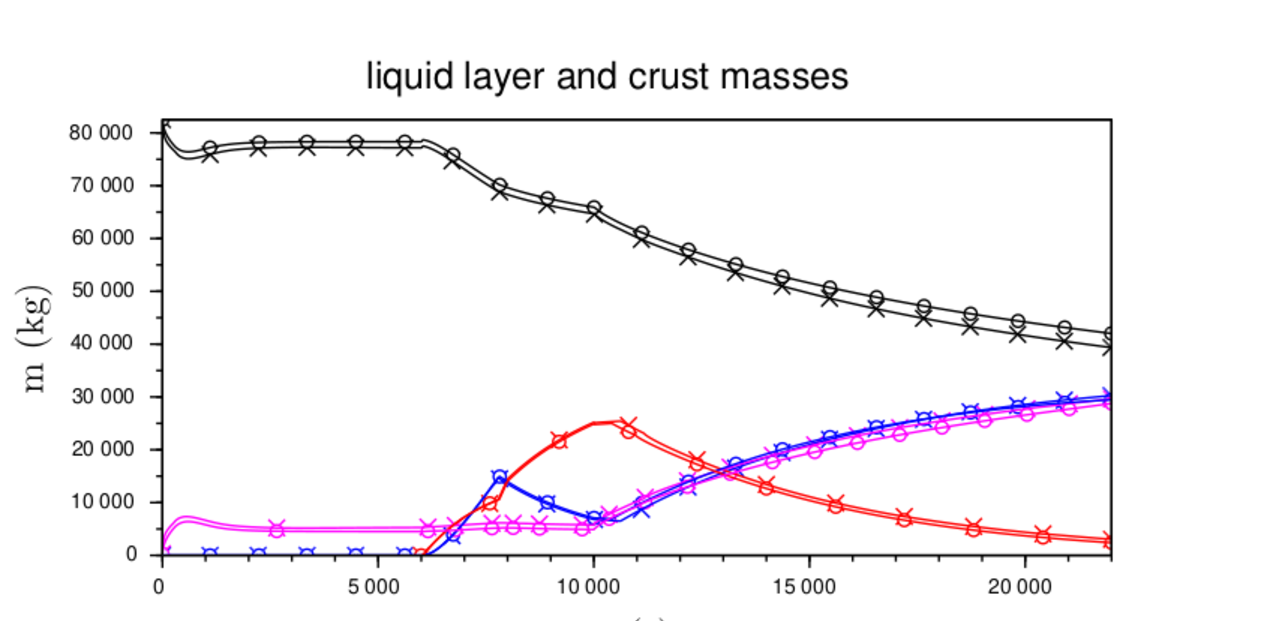
\includegraphics[width=0.47\textwidth]{Figures/IndustrialTestmasses2.pdf}
    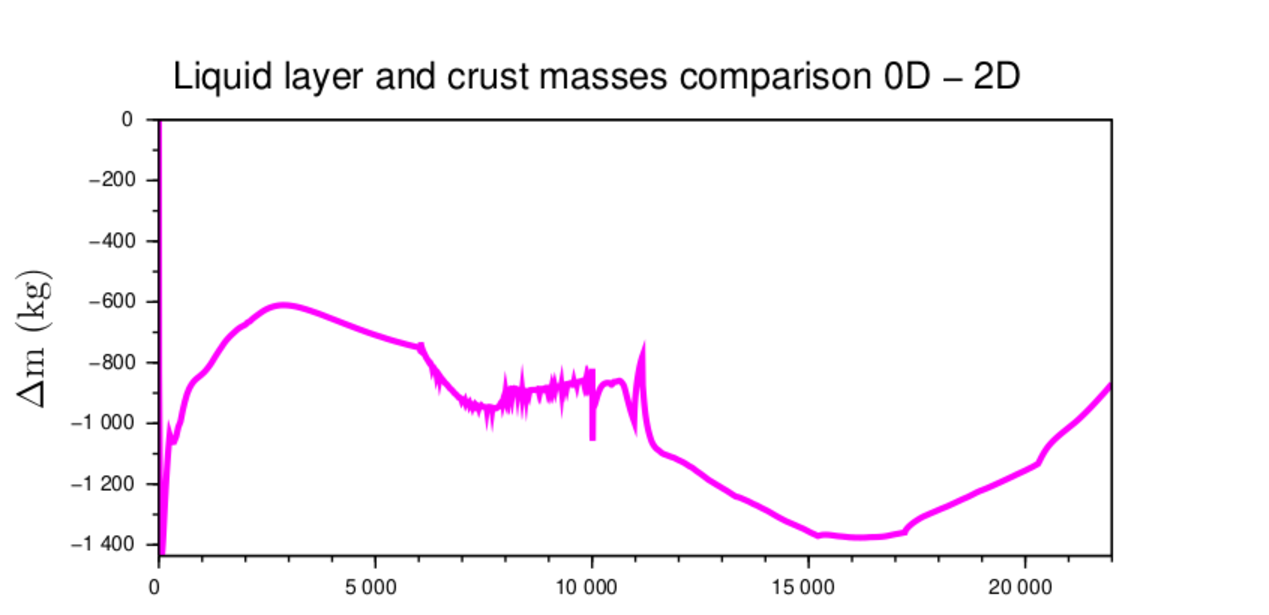
\includegraphics[width=0.47\textwidth]{Figures/IndustrialTestdiffMasses2.pdf}\\

 \center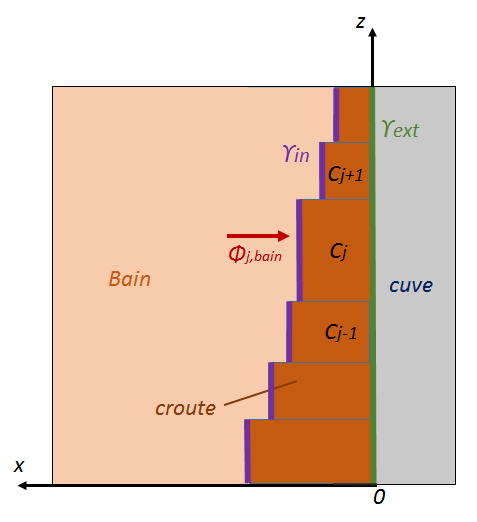
\includegraphics[width=0.3\textwidth]{Figures/modele_croute_0D.png}
 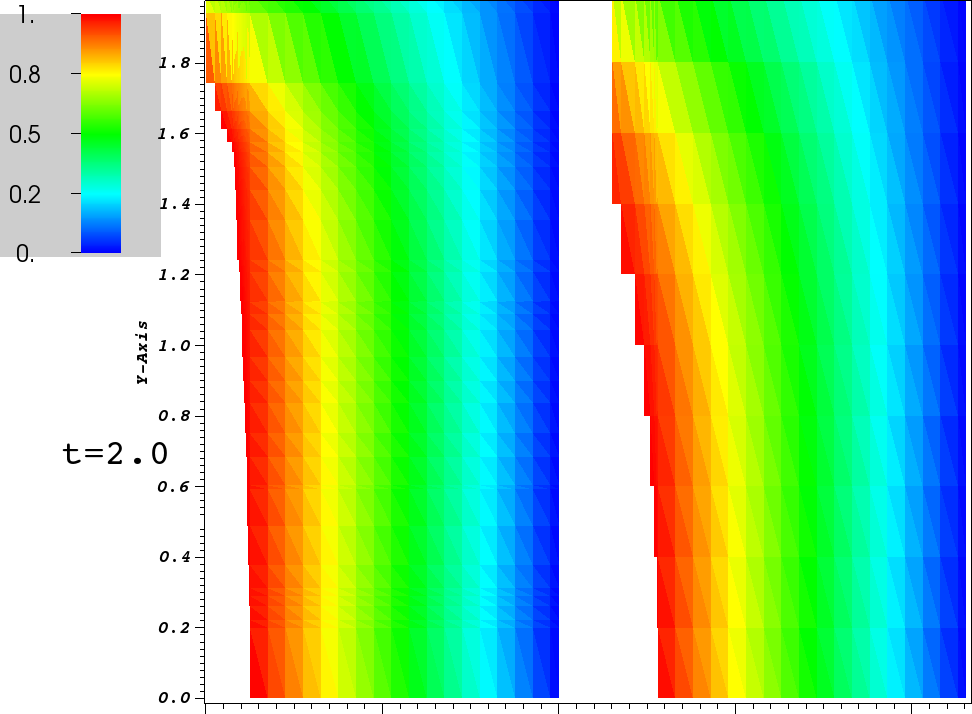
\includegraphics[width=0.35\textwidth]{Figures/Full2D_Bi1_2_t200002.png}
    
\end{frame}
%--------------------------------------------------------------------------
%==========================================================================
%--------------------------------------------------------------------------
\Intercalaire{Prise en compte plus fine du bain de corium par une approche CFD et un modèle d'interface VOF/FT}
\section{Prise en compte plus fine du bain de corium par une approche CFD et un modèle d'interface VOF/FT}
\subsection{Environnement de travail}
\subsection{Présentation de la méthode VOF/FT et des adaptations apportées}
\subsection{Résultats de validation et cas test de la couche mince}


\begin{frame}
    \frametitle{Équations considérées}
\footnotesize
\color{cea_rouge} \underline{Navier-Stokes + transfert de chaleur avec changement de phase à l'interface $\Gamma$ :}  \color{cea_texte}
\begin{align}
	 (\mathcal{P})  &: \left\{ {\hlTab{2}\begin{array}{l} 
	\rho \frac{\partial  \vect{u}}{\partial t} +\rho \vect{u} \nabla  \vect{u} = -\nabla P + \rho \vect{g} + \vect{\mathcal{D}},\\
	\nabla \cdot \vect{u} = \color{red} - \Dot{m} \left( \frac{1}{\rho_l} - \frac{1}{\rho_s} \right) \delta^\Gamma,\\
	\frac{\partial \rho C_p \delta T}{\partial t} +\nabla \cdot (\rho \vect{u} C_p \delta T) = \nabla \cdot (\lambda \nabla T)\color{red} +  \Dot{m} \Delta \mathcal{H}^\Gamma \delta^\Gamma,\\
	\frac{\partial \chi}{\partial t} + \vect{u^\inte} \cdot \nabla \chi =0,
	 \end{array}}\right.
\end{align}
 avec pour tout $\vect{x}$ dans $\Gamma$ :
\begin{align}
	\vect{u}^\inte&= \color{red} - \frac{\Dot{m}}{\rho_s} \norm^\inte \color{black}\color{black}, 
\end{align}
et  :
\begin{align}
	\Dot{m} &= \frac{\varphi_l - \varphi_s}{ \Delta \chaL^\Gamma} .
\end{align}
Dans ce système les inconnues sont  la vitesse $\vect{u}$, la pression $P$, la température $T$ et la fonction $\chi$.
\end{frame}

\begin{frame}
    \frametitle{Équations considérées : fermeture à l'interface}
\footnotesize


\begin{center}
		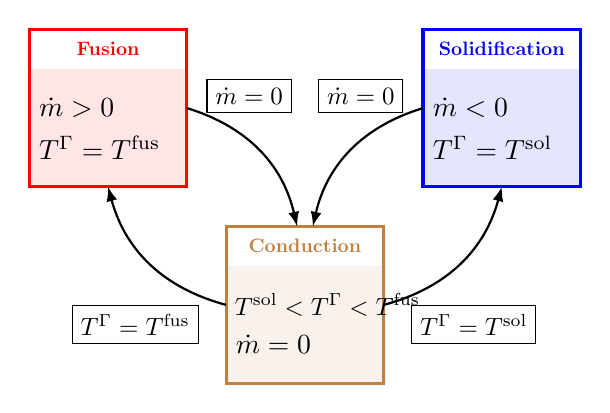
\begin{tikzpicture}[scale = 0.5, every node/.style={scale=0.5}]
			\fill[red!10] (-5,5) rectangle (-1,8);
\fill[blue!10] (5,5) rectangle (9,8);
\fill[brown!10] (0,0) rectangle (4,3);
\draw[red, very thick] (-5,5) rectangle (-1,9);
\draw[brown, very thick] (0,0) rectangle (4,4);
\draw[blue, very thick] (5,5) rectangle (9,9);


\draw (-3, 8.5) node[red , scale=1.4, align =left]{ \textbf{Fusion}};
\draw (7, 8.5) node[blue , scale=1.4, align =left]{ \textbf{Solidification}};
\draw (2, 3.5) node[brown , scale=1.4, align =left]{ \textbf{Conduction}};

\draw (-5, 7.) node[ scale=2,right,align =left]{ $\Dot{m} > 0$};
\draw (-5, 6.) node[ scale=2,right,align =left]{ $T^\Gamma = T^\fus$};

\draw (5, 7.) node[ scale=2,right,align =left]{ $\Dot{m} < 0$};
\draw (5, 6.) node[ scale=2,right,align =left]{ $T^\Gamma = T^\sol$};


\draw (0, 2) node[ scale=1.8,right,align =left]{ $T^\sol<T^\Gamma < T^\fus$ };
\draw (0, 1.) node[ scale=2,right,align =left]{ $ \Dot{m} = 0$};


\draw[->,>=latex, black, thick] (-1., 7) to[bend left] (1.8, 4);
\draw[->,>=latex, black, thick] (5, 7) to[bend right] (2.2, 4);

\draw[->,>=latex, black, thick] (0, 2) to[bend left] (-3, 5);
\draw[->,>=latex, black, thick] (4, 2) to[bend right] (7, 5);

\draw (-0.5, 7.3) node[rectangle, draw,right, scale=1.8]{ $\Dot{m} = 0$};
\draw (4.5, 7.3) node[rectangle, draw,left, scale=1.8]{ $\Dot{m} = 0$};

\draw (-0.7, 1.5) node[rectangle, draw,left, scale=1.8]{ $T^\Gamma = T^\fus$};
\draw (4.7, 1.5) node[rectangle, draw,right, scale=1.8]{ $T^\Gamma = T^\sol$};

		\end{tikzpicture}

\end{center}
\begin{ceablock}{Trois lois de fermetures thermiques à l'interface en fonction de "son état" :}
\begin{align}
	(\mathcal{F}) &:\left\{ \begin{array}{ll}
T=T^\sol,  \; &\text{ si } \Dot{m} \leq 0, \\
\vect{\varphi}_s \cdot \norm^\inte= \vect{\varphi}_l \cdot \norm^\inte,  \; &\text{ si } T^\sol < T^\inte < T^\fus,\\
T=T^\fus,   \; &\text{ si } \Dot{m}>0.
 \end{array}\right.
\end{align}
\end{ceablock}
\end{frame}


\begin{frame}
    \frametitle{Présentation du code TrioCFD}
    \footnotesize
    \begin{itemize}
    \item \textbf{Résolution de Navier-Stokes incompressible} par méthode de prédiction-projection
        \item \textbf{Discrétisations spatiales} \bib{TrioCFD} :\\
            $\bullet$ Volumes Différences finies (VDF) : rectangle en 2D, hexaèdre en 3D.\\
            $\bullet$ Volumes Éléments Finis (VEF) : triangle en 2D, tétraèdre/hexahèdre en en 3D .
        
 %       \item Schéma semi-implicite "SIMPLE" (seul les termes de diffusion sont implicités)
%        \item Schéma implicite
    \end{itemize}
    
\begin{columns}[c]
	\begin{column}{0.4\textwidth}
\begin{center}
		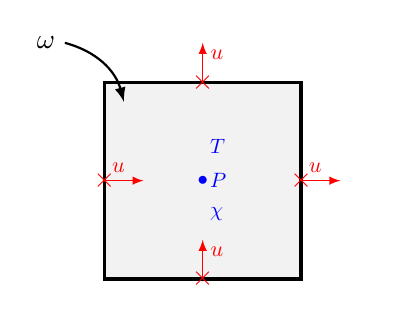
\begin{tikzpicture}[scale = 0.5, every node/.style={scale=0.5}]
			
\fill[gray!10!](0,0) rectangle (5,5);
\draw[very thick](0,0) rectangle (5,5);


%normal
\draw[->,>=latex, red] (0, 2.5) to (1, 2.5);
\draw[->,>=latex, red] (5, 2.5) to (6, 2.5);
\draw[->,>=latex, red] (2.5, 0) to (2.5, 1);
\draw[->,>=latex, red] (2.5, 5) to (2.5, 6);


\draw (2.5, 2.5) node[blue,scale=1.5]{$\bullet$};
\draw (2.5,0) node[red, scale=2]{$\times$};
\draw (2.5,5) node[red, scale=2]{$\times$};
\draw (0,2.5) node[red, scale=2]{$\times$};
\draw (5,2.5) node[red, scale=2]{$\times$};

\draw (2.5, 3) node[blue,scale=1.5, above right]{$T$};
\draw (2.5, 2.5) node[blue,scale=1.5,  right]{$P$};
\draw (2.5, 2) node[blue,scale=1.5, below right]{$\chi$};

\draw(5.,2.5) node[red,scale =1.6, above right]{$u$};
\draw(0.,2.5) node[red,scale =1.6, above right]{$u$};

\draw(2.5,0.7) node[red,scale =1.6, right]{$u$};
\draw(2.5,5.7) node[red,scale =1.6, right]{$u$};

\draw[->,>=latex, black, thick] (-1,6) to[bend left] (.5, 4.5);
\draw(-1,6) node[scale =2, left]{$\omega$};

\draw(6,6) node[scale =2, right, white]{$\omega$};

		\end{tikzpicture}
\end{center}
\end{column}
\begin{column}{0.6\textwidth}
\begin{ceablock}{Interface : plusieurs méthodes disponibles. }
\begin{itemize}
	\item Une \textbf{méthode VOF/FT } : pour des interfaces de changement de phase entre liquide-vapeur. 
	\item Une \textbf{méthode de pénalisation} sans changement de phase (modélisation d'un agitateur en fond de bécher).
	\item Une  \textbf{méthode Ghost-Fluid} pour la résolution de la température.
\end{itemize}
\end{ceablock}
\end{column}
\end{columns}
\vspace{0.3cm}
\fbox{\begin{minipage}[]{\textwidth}
\begin{center}
\textcolor{red}{$\Rightarrow$ Adapter la méthode VOF-FT pour suivre l'interface liquide-solide.\\
 $\Rightarrow$ Vérifier la compatibilité de la méthode de pénalisation avec le changement de phase.\\
 $\Rightarrow$ Adapter la méthode ghost-fluid aux nouveaux états d'interface.}
\end{center}
\end{minipage}}
\end{frame}


\begin{frame}
    \frametitle{Méthode VOF--Front-Tracking}
    \footnotesize
    \begin{columns}[c]
    \begin{column}{0.6 \textwidth}
    \begin{ceablock}{La méthode Front-Tracking \bib{Tryggvason et al.} :}
        \begin{itemize}
            \item Méthodes d'interpolation nécessaires pour communiquer  d'un maillage à l'autre.
            \item \textbf{Pas naturellement conservative}.
            \item Algorithmie difficile à mettre en place.
        \end{itemize}
    \end{ceablock}
\begin{ceablock}{La méthode Volume Of Fluid \bib{Benson} :}
        \begin{itemize}
            \item Méthode eulérienne, basée sur une fonction de fraction de présence.
            \item \textbf{Conservative} par construction.
            \item Pas de suivi de l'interface, besoin d'algorithme de reconstruction.
            
        \end{itemize}
    \end{ceablock}
\end{column}
\begin{column}{0.4 \textwidth}
\begin{center}
		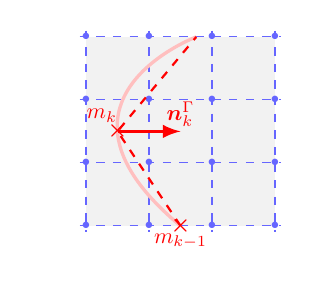
\begin{tikzpicture}[scale = 0.4, every node/.style={scale=0.4}]
			


%\fill[gray!10!](2,3) -- (8,3) -- (8,2) -- (9,2) -- (9,1) --(10,1) -- (10, -1) -- (9,-1) -- (9,-2) -- (8,-2) -- (8,-3) -- (2,-3) -- (2,-2) -- (1,-2) -- (1, -1) -- (0,-1) -- (0,1) -- (1,1) -- (1,2) -- (2,2) -- cycle;
%\draw[very  thick](2,3) -- (8,3) -- (8,2) -- (9,2) -- (9,1) --(10,1) -- (10, -1) -- (9,-1) -- (9,-2) -- (8,-2) -- (8,-3) -- (2,-3) -- (2,-2) -- (1,-2) -- (1, -1) -- (0,-1) -- (0,1) -- (1,1) -- (1,2) -- (2,2) -- cycle;

%interface
%\draw[red!25!, very thick] (5,3) ..controls +(2,-1) and +(0,2).. (6,0);
%\draw[red!25!, very thick] (6,0) ..controls +(0,-2) and +(-3,2).. (5,-3);


% maillage carte




%\draw[black, dashed, thick] (4.5,-2) circle (1.5);
%\draw[->,>=latex, black] (6, -2) to (12.5, -3);

\fill[gray!10!] (13,0) rectangle (19,-6);

\draw[blue!60, dashed](12.8,0) -- (19.2,0);
\draw[blue!60, dashed, dashed](12.8,-2) -- (19.2,-2);
\draw[blue!60, dashed](12.8,-4) -- (19.2,-4);
\draw[blue!60, dashed](12.8,-6) -- (19.2,-6);



\draw[blue!60, dashed](13.,0.2) -- (13,-6.2);
\draw[blue!60, dashed](15.,0.2) -- (15,-6.2);
\draw[blue!60, dashed](17.,0.2) -- (17,-6.2);
\draw[blue!60, dashed](19.,0.2) -- (19,-6.2);


\foreach \x in { 13 ,15, 17, 19}
    \draw (\x, 0) node[blue!60, scale =1.5]{ $\bullet$};
\foreach \x in { 13 ,15, 17, 19}
    \draw (\x, -2) node[blue!60, scale =1.5]{ $\bullet$};
\foreach \x in { 13 ,15, 17, 19}
    \draw (\x, -4) node[blue!60, scale =1.5]{ $\bullet$};
\foreach \x in { 13 ,15, 17, 19}
    \draw (\x, -6) node[blue!60, scale =1.5]{ $\bullet$};





%noral


% Maillage interface

%\draw (5, 3) node[red, scale=2]{$\bm{\times}$};
%\draw (6.25, 1.8) node[red, scale=2]{$\bm{\times}$};
%\draw (6,0) node[red, scale=2]{$\bm{\times}$};
%\draw (3.9, -2) node[red, scale=2]{$\bm{\times}$};
%\draw (5, -3) node[red, scale=2]{$\bm{\times}$};

%\draw[red, dashed, thick](5, 3) -- (6.25, 1.8) -- (6,0) -- (3.9, -2) -- (5, -3);


\draw[red!25!, very thick] (16, -6) ..controls +(-4.8,4) and +(-0,0).. (16.5, 0);
\draw (14, -3) node[red, scale=2]{$\bm{\times}$};
\draw (16, -6) node[red, scale=2]{$\bm{\times}$};
\draw[red, dashed, thick](16, -6) -- (14, -3) -- (16.5, 0);

%\draw (4.1, -2) node[red, scale=2, right]{$m_k$};
%\draw (6, -3.2) node[red, scale=2, below]{$m_{k-1}$};
%\draw (6,0) node[red, scale=2, right]{$m_{k+1}$};
%\draw  (6.25, 1.5) node[red, scale=2, right]{$m_{k+2}$};
%\draw (5, 3.2) node[red, scale=2, above]{$m_{k+3}$};


\draw (16, -6) node[red, scale=2, below]{$m_{k-1}$};
\draw (13.5, -2.5) node[red, scale=2]{$m_{k}$};

\draw[->,>=latex, red, very thick] (14, -3) to (16, -3);
\draw (16, -3.1) node[red, scale=2, above]{$\bm{n}_{k}^\Gamma$};

		\end{tikzpicture}

\end{center}
\begin{center}
		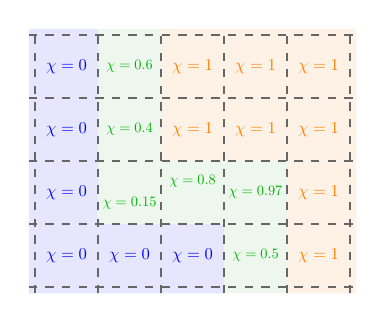
\begin{tikzpicture}[scale = 0.4, every node/.style={scale=0.4}]
			
\fill[blue!95!gray!10] (-0.2,-0.2) -- (-0.2,8.2) -- (2,8.2) -- (2,2) -- (6,2) -- (6,-0.2)  -- cycle;
\fill[orange!95!gray!10] (4,8.2) -- (10.2,8.2) -- (10.2,-0.2) -- (8,-0.2) -- (8,4) -- (4,4)  -- cycle;
\fill[green!35!gray!10] (2,8.2) -- (4,8.2) -- (4,4) -- (2,4)  -- cycle;
\fill[green!35!gray!10] (2,4) rectangle (6,2);
\fill[green!35!gray!10] (6,4) rectangle (8,-0.2);


\foreach \x in { 0, 2, 4, 6, 8}
    \draw[black!60, thick, dashed](-0.2,\x) -- (10.2,\x);

\foreach \x in { 0, 2, 4, 6, 8, 10}
   \draw[black!60, thick, dashed](\x,-0.2) -- (\x,8.2);




%\draw (2.7,8.5) node[red, above, scale=1.5]{$\Gamma$};


%\draw[very thick,red ](2.7,8.5) -- (3.3,4);
%\draw[very thick,red](3.3,4) -- (3.4,3.25) -- (6.0, 2.2);
%\draw[very thick,red](6.0, 2.2) -- (6.2, 2.11) -- (7.8, -0.2) ;

%\draw (3.4,3.25) node[ scale=2]{$\bm{\times}$};
%\draw (6.2, 2.11) node[ scale=2]{$\bm{\times}$};




\draw (1,1) node[blue, scale=1.5]{$\chi=0$};
\draw (3,1) node[blue, scale=1.5]{$\chi=0$};
\draw (5,1) node[blue, scale=1.5]{$\chi=0$};
\draw (1,3) node[blue, scale=1.5]{$\chi=0$};
\draw (1,5) node[blue, scale=1.5]{$\chi=0$};
\draw (1,7) node[blue, scale=1.5]{$\chi=0$};

\draw (9,7) node[orange, scale=1.5]{$\chi=1$};
\draw (9,5) node[orange, scale=1.5]{$\chi=1$};
\draw (9,3) node[orange, scale=1.5]{$\chi=1$};
\draw (9,1) node[orange, scale=1.5]{$\chi=1$};
\draw (7,7) node[orange, scale=1.5]{$\chi=1$};
\draw (5,7) node[orange, scale=1.5]{$\chi=1$};
\draw (7,5) node[orange, scale=1.5]{$\chi=1$};
\draw (5,5) node[orange, scale=1.5]{$\chi=1$};


\draw (3,7) node[black!30!green!99, scale=1.3]{$\chi=0.6$};
\draw (3,5) node[black!30!green!99, scale=1.3]{$\chi=0.4$};
\draw (3,3) node[below, black!30!green!99, scale=1.3]{$\chi=0.15$};
\draw (5,3) node[black!30!green!99,above, scale=1.3]{$\chi=0.8$};
\draw (7,3) node[black!30!green!99, scale=1.3]{$\chi=0.97$};
\draw (7,1) node[black!30!green!99, scale=1.3]{$\chi=0.5$};



		\end{tikzpicture}

\end{center}
\end{column}
\end{columns}
\end{frame}

\begin{frame}
    \frametitle{Couplage des équations}
        %\textbf{Schéma en temps explicite} : Résolution de la vitesse du fluide, déplacement des marqueurs et mise à jour de la fonction $\chi_v$, résolution de la température.
        \footnotesize
        \begin{ceablock}{Résolution séquentielle explicite :}
        \begin{itemize}
            \item Résolution de la vitesse du fluide $\vect{u}$ et de la pression $P$.\\
				\color{cea_texte!70}$\bullet$ Méthode de prédiction-projection avec divergence nulle.\\
				$\bullet$ Ajout de la méthode de pénalisation, avec divergence nulle.\\
				$\bullet$ Prise en compte du terme de divergence non nulle.\color{cea_texte}
			
            \item Déplacement des marqueurs et mise à jour de la fonction $\chi$.
            \item Résolution de la température $T$.\\
            	\color{cea_texte!70}$\bullet$ Méthode ghost-fluid sans prise en compte des états d'interface.\\
            	$\bullet$ Adaptation  à la notion d'états d'interfaces.           
        \end{itemize}
        \end{ceablock}
    
\end{frame}

\begin{frame}
    \frametitle{Résolution de la vitesse : méthode de prédiction-projection}
    \footnotesize
    \begin{ceablock}{Résolution de la vitesse sur tout le domaine par une méthode de prédiction-projection :}
	\textbf{Prédiction :}
	\begin{align} 
		\vect{u}^* &= \vect{u}^n - \Delta t \nabla_h \cdot (\vect{u}^n \vect{u}^n) + \frac{\Delta t}{\rho^n_f} \nabla_h \cdot(\mu^n(\nabla_h \vect{u}^n+\nabla^T_h \vect{u}^n)),
	\end{align}
	\color{cea_texte!70}où $\vect{u}^*$ est la prédiction de la vitesse, $\mu^n$ la viscosité discrète, et où $\rho^n_f$ la masse volumique discrète aux faces. $\nabla_h$ est la divergence discrète. \color{cea_texte}\\  %(obtenue par interpolation linéaire)
	\vspace{0.3cm}

	\textbf{Projection :}
rajout de la contribution de la pression $P^\npl$ $\Rightarrow$ vitesse à divergence nulle.

	\begin{align}
		\vect{u}^{n+1} &= \vect{u}^* + \frac{\Delta t}{\rho^n_f} \nabla_h P^{n+1},
	\end{align}
	\color{cea_texte!70}où, $P^{n+1}$ est obtenue en résolvant : \color{cea_texte}
\begin{align}
\label{eq:Pression}
					 \nabla_h \cdot  \left( \frac{1}{\rho^n_f} \nabla_h P^\npl \right) &=  -\frac{1}{\Delta t} \nabla_h \cdot \vect{u}^*. 
\end{align}
	\end{ceablock}

\end{frame}

\begin{frame}
    \frametitle{Résolution de la vitesse : la méthode de pénalisation}
    \footnotesize
     \footnotesize
        \begin{ceablock}{Modification de l'algorithme initial pour imposer une vitesse nulle sur le solide :}
	Utilisation de la méthode de pénalisation, déjà présente dans TrioCFD \bib{Belliard et al.}
\begin{align}
	\vect{I}^n &= \nabla_h \cdot (\vect{u}^n \vect{u}^n) + \frac{1}{\rho^n} \nabla_h \cdot(\mu^n(\nabla_h \vect{u}^n+\nabla_h^T \vect{u}^n)).
\end{align}
	\textbf{Prédiction :}
\begin{align}
	(1+\frac{\chi}{\eta} ) \vect{u}^* &= \vect{u}^n + \Delta t \vect{I}^n, \label{eq:PDFpred1} \\ 
	\vect{u}^* &= \frac{\vect{u}^n + \Delta t \vect{I}^n}{(1+\frac{\chi}{\eta} )}. \label{eq:PDFpred2}
\end{align}
	où $\eta$ est le facteur de pénalisation très proche de $0$, $\eta=10^{-12}$.
	

	\textbf{Projection :}

\begin{align}
	\vect{u}^{n+1} &= \vect{u}^* + \frac{\Delta t}{\rho^n_f} \nabla_h P^{n+1} +\frac{\chi}{\eta}(\vect{u}^*-\vect{u}^\npl),\\
-\nabla_h \cdot \vect{u}^* &= \Delta t \, \frac{\eta}{\eta + \chi} \nabla_h \cdot \left( \frac{1}{\rho^n_f} \nabla_h P^\npl \right) \underset{\eta \to 0}{\longrightarrow} 0.
%
%	\frac{\eta}{\eta + \chi} \nabla_h \cdot \left( \frac{1}{\rho^n_f} \nabla_h P^\npl \right) &= -\frac{1}{\Delta t} \nabla_h \cdot \vect{u}^* .
\end{align}
	\end{ceablock}

\end{frame}

\begin{frame}
    \frametitle{Résolution de la vitesse : discrétisation de la divergence}
    \footnotesize
        Prise en compte de la contribution du changement de volume à \textbf{divergence non-nulle}.\\
\begin{align}
	 \int_\omega \zeta (t) dx &= \int_{\inte (t) \cap \omega} \Dot{m}(t) \left( \frac{1}{\rho_l} - \frac{1}{\rho_s} \right) d\sigma dt.
\end{align}

\color{cea_rouge}\underline{Discrétisation :}\color{cea_texte}
\begin{align}
	\zeta^n &= \frac{\normeVec{\inte^n \cap \omega}}{\normeVec{\omega}}\Dot{m}^n \left( \frac{1}{\rho_l} - \frac{1}{\rho_s} \right).
\end{align}
\color{cea_rouge}\underline{Modification de l'espace de projection :}\color{cea_texte}
\begin{align}
	\label{eq:pression3}
	\frac{\eta}{\eta + \chi} \nabla_h \cdot \left( \frac{1}{\rho^n_f} \nabla_h P^\npl \right) &= -\frac{1}{\Delta t} \nabla_h \cdot \vect{u}^* + \frac{1}{\Delta t} \zeta^n.
\end{align}
\vspace{0.3cm}

\begin{center}
		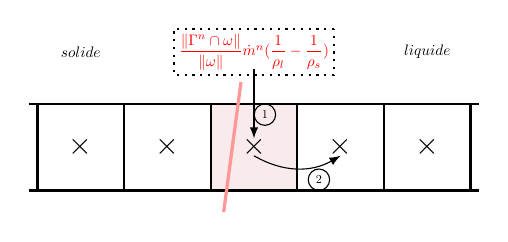
\begin{tikzpicture}[scale = 0.55, every node/.style={scale=0.55}]
			%\fill[gray!10] (-0.2,0) -- (-0.2,2) -- (10.2,2) -- (10.2,0)  -- cycle;
\fill[red!55!gray!10] (4,0) -- (4,2) -- (6,2) -- (6,0)  -- cycle;
\draw[ thick](-0.2,0) -- (10.2,0);
\draw[ thick](-0.2,2) -- (10.2,2);

\draw[ thick](0.,0) -- (0,2);
\draw[ thick](2.,0) -- (2,2);
\draw[ thick](4.,0) -- (4,2);
\draw[ thick](6.,0) -- (6,2);
\draw[ thick](8.,0) -- (8,2);
\draw[ thick](10.,0) -- (10,2);

\draw (1, 1) node[ scale=2]{$\times$};
\draw (3, 1) node[ scale=2]{$\times$};
\draw (5, 1) node[ scale=2]{$\times$};
\draw (7, 1) node[ scale=2]{$\times$};
\draw (9, 1) node[ scale=2]{$\times$};

%\draw (5, 0.5) node[ scale=1]{$d_0$};
%\draw (7, 0.5) node[ scale=1]{$d_1$};
%\draw (9, 0.5) node[ scale=1]{$d_2$};
%\draw (3, 0.5) node[ scale=1]{$d_{-1}$};
%\draw (1, 0.5) node[ scale=1]{$d_{-2}$};

%\draw (4, 2.2) node[ scale=1]{$\alpha_0$};
%\draw (6, 2.2) node[ scale=1]{$\alpha_1$};
%\draw (8, 2.2) node[ scale=1]{$\alpha_2$};
%\draw (10, 2.2) node[ scale=1]{$\alpha_3$};
%\draw (2, 2.2) node[ scale=1]{$\alpha_{-1}$};
%\draw (0, 2.2) node[ scale=1]{$\alpha_{-2}$};
%\textcircled
\draw (1, 3.2) node[ scale=1]{$solide$};
\draw (9, 3.2) node[ scale=1]{$liquide$};
\draw (5, 3.2) node[rectangle,draw,thick,dotted, scale=1]{$\color{red} \frac{\normeVec{\inte^n \cap \omega}}{\normeVec{\omega}}\Dot{m}^n (\frac{1}{\rho_l}-\frac{1}{\rho_s})$};

\draw[->,>=latex] (5, 2.8) to (5, 1.2);
\draw (5, 1.75) node[circle,draw,right, scale=0.8]{$1$};
\draw[->,>=latex] (5, 0.8) to[bend right] (7, 0.8);
\draw (6.5, 0.5) node[circle,draw,below, scale=0.8]{$2$};
\draw[very thick, red!40](4.3,-0.5) -- (4.7,2.5);

		\end{tikzpicture}
\end{center}
\end{frame}

\begin{frame}
    \frametitle{Résolution du modèle de l'interface}
    \footnotesize
Calcul de la vitesse d'interface $\vect{u}^\inte$ :
\begin{align}
	\label{eq:interfaceVitesse}
	\vect{u}^{\inte,n} &=  - \nabla \cdot \left( \frac{\Dot{m}^n}{\rho_s}d^n \right),
\end{align}
\begin{enumerate}
	\item Advection théorique  des fractions volumiques (fonction couleur $\chi$).
	\item Déplacements des marqueurs.
	\item Algorithme de remaillage, lissage, barycentrage.
	\item Correction du déplacement des marqueurs à l'aide de la fonction $\chi$.
	\item Mise en cohérence de la fonction $\chi$ en fonction des marqueurs.
	\item Mise à jour de la fonction level-set $d$, représentant la distance signée à l'interface.

\end{enumerate}
\end{frame}

\begin{frame}
    \frametitle{Résolution de la température : méthode Ghost-Fluid}
    	\footnotesize
\begin{ceablock}{Séparation de l'équation de température en deux équations, une pour chaque phase :}
\begin{align}
 (\delta T_k^\npl)   = (\delta T^n_k) + \frac{\lambda_k \Delta t }{\rho_k C_{p,k}}  \Delta_h T_k^n - \Delta t \nabla_h \cdot ( \vect{u}^{T,n} \delta T_k^n), \quad k=l,s.
\end{align}
définies sur tout le domaine. 
\end{ceablock}
\vspace{0.3cm}
\begin{ceablock}{Propagation de la température en accord avec $T^\inte$ par méthode la Ghost-Fluid :}
1/ Calcul d'un \textbf{gradient de chaleur normal} à l'interface aux  centres des mailles solides.
\begin{align}
 (\ghost T_s \cdot \norm) &= \frac{T^\inte - T_s}{d}.
\end{align}
\end{ceablock}
2/ \textbf{Extrapolation du gradient} aux mailles mixtes et liquides proches de l'interface.
\begin{center}
		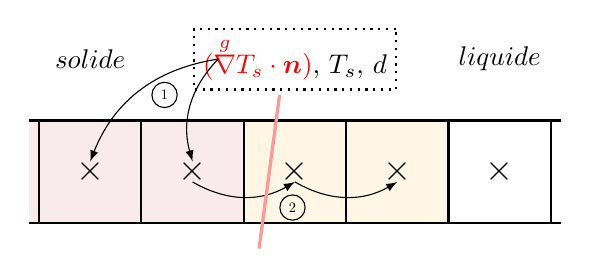
\begin{tikzpicture}[scale = 0.65, every node/.style={scale=0.65}]
			\fill[red!55!gray!10] (-0.2,0) -- (-0.2,2) -- (4,2) -- (4,0)  -- cycle;
\fill[red!35!yellow!10] (4,0) rectangle (8,2);
\draw[ thick](-0.2,0) -- (10.2,0);
\draw[ thick](-0.2,2) -- (10.2,2);

\draw[ thick](0.,0) -- (0,2);
\draw[ thick](2.,0) -- (2,2);
\draw[ thick](4.,0) -- (4,2);
\draw[ thick](6.,0) -- (6,2);
\draw[ thick](8.,0) -- (8,2);
\draw[ thick](10.,0) -- (10,2);

\draw (1, 1) node[ scale=2]{$\times$};
\draw (3, 1) node[ scale=2]{$\times$};
\draw (5, 1) node[ scale=2]{$\times$};
\draw (7, 1) node[ scale=2]{$\times$};
\draw (9, 1) node[ scale=2]{$\times$};

%\draw (5, 0.5) node[ scale=1]{$d_0$};
%\draw (7, 0.5) node[ scale=1]{$d_1$};
%\draw (9, 0.5) node[ scale=1]{$d_2$};
%\draw (3, 0.5) node[ scale=1]{$d_{-1}$};
%\draw (1, 0.5) node[ scale=1]{$d_{-2}$};

%\draw (4, 2.2) node[ scale=1]{$\alpha_0$};
%\draw (6, 2.2) node[ scale=1]{$\alpha_1$};
%\draw (8, 2.2) node[ scale=1]{$\alpha_2$};
%\draw (10, 2.2) node[ scale=1]{$\alpha_3$};
%\draw (2, 2.2) node[ scale=1]{$\alpha_{-1}$};
%\draw (0, 2.2) node[ scale=1]{$\alpha_{-2}$};
%\textcircled
\draw (1, 3.2) node[ scale=1.5]{$solide$};
\draw (9, 3.2) node[ scale=1.5]{$liquide$};
\draw (5, 3.2) node[rectangle,draw,thick,dotted, scale=1.5]{$\color{red} (\ghost T_s \cdot \norm)$, $\color{black} T_s$, $d$};


\draw[->,>=latex] (3.5, 3.2) to[bend right] (1, 1.2);
\draw[->,>=latex] (3.5, 3.2) to[bend right] (3, 1.2);

\draw (2.2, 2.5) node[circle,draw,right, scale=0.8]{$1$};

\draw[->,>=latex] (5, 0.8) to[bend right] (7, 0.8);
\draw[->,>=latex] (3, 0.8) to[bend right] (5, 0.8);
\draw (4.7, 0.3) node[circle,draw,right, scale=0.8]{$2$};

\draw[very thick, red!40](4.3,-0.5) -- (4.7,2.5);

		\end{tikzpicture}

\end{center}
\end{frame}

\begin{frame}
    \frametitle{Résolution de l'équation de la chaleur : états  et température d'interface}
   	\footnotesize
\begin{enumerate}
	\item Nouveau champ  eulérien : "\textbf{états d'interface}" $E^n\rightarrow E^\npl$
\begin{align}
\label{eq:etatn2}
E^\npl &=\left\{ {\renewcommand{\arraystretch}{1.5}\begin{array}{ll} 
\text{conduction} &\text{ si } T^\sol < T^{\Gamma,n} <T^\fus,\\
\text{conduction} &\text{ si } E^n = \text{fusion} \text{ et } \dot{m}<0,\\
\text{conduction} &\text{ si } E^n = \text{solidification} \text{ et } \dot{m}>0,\\
\text{fusion} &\text{ si } T^{\Gamma,n} \geq T^\fus \text{ et } \dot{m} \geq 0,\\
\text{solidification} &\text{ si } T^{\Gamma,n} \leq T^\sol \text{ et } \dot{m} \leq 0.
 \end{array}}\right.
\end{align}
Extrapolation aux mailles pures proches.
\item Calcul de la   \textbf{température d'interface}, comme fonction de l'état de la maille $E^\npl$:
\begin{align}
	T^{\inte, \npl} &= \left\{ {\renewcommand{\arraystretch}{1.}\begin{array}{l l l} 
		T^\fus & \text{ si } E^\npl =\text{fusion},\\
		T^{\text{cond}} & \text{  si } E^\npl = \text{  conduction},\\
		T^\sol & \text{ si } E^\npl = \text{ solidification}.
 \end{array}}\right.
\end{align} 





\end{enumerate}
\center\fbox{\begin{minipage}[]{0.8\textwidth}
\begin{center}
 \textcolor{red}{$T^{\cond}$ reste à déterminer en fonction des profils de température.}
\end{center}
\end{minipage}}
\end{frame}


\begin{frame}
    \frametitle{Calcul de $ T^{\cond}$}
    \footnotesize
Calcul de $T^{\text{cond}}$ via l'\textbf{égalité des flux de chaleur}.
    \begin{align}
  \vect{\varphi}_s \cdot \norm^\inte= \vect{\varphi}_l \cdot \norm^\inte \quad \Rightarrow \quad \lambda_s \Frac{T^{\text{cond}}- \overline{T_s}}{\overline{d_s}} &= \lambda_l \Frac{\overline{T_l}-T^{\text{cond}}}{-\overline{d_l}} 
\end{align}
%    \begin{align}
%    T^{\text{cond}} &= \Frac{\lambda_s \overline{T_s} \, \overline{d_l} - \lambda_l \overline{T_l}  \, \overline{d_s}}{\lambda_s \overline{d_l} - \lambda_l \overline{d_s}}.
%\end{align}

\textcolor{cea_texte!70}{où $\overline{T_k}$ est la température moyenne et  $\overline{d_k}$ la distance moyenne à l'interface  pour la phase $k$.}
\begin{columns}[c]
    \begin{column}{0.5 \textwidth}
\begin{center}
		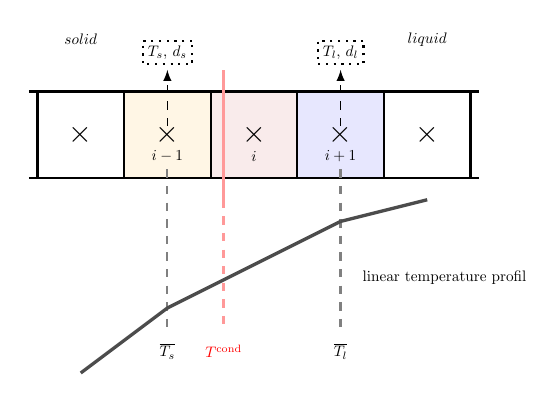
\begin{tikzpicture}[scale = 0.55, every node/.style={scale=0.55}]
			
%\fill[gray!10] (-0.2,0) -- (-0.2,2) -- (10.2,2) -- (10.2,0)  -- cycle;
\fill[red!55!gray!10] (4,2) -- (4,0)  -- (6,0) -- (6,2) -- cycle;
\fill[blue!90!gray!10] (6,0) rectangle (8,2);
\fill[red!35!yellow!10] (2,0) rectangle (4,2);
\draw[ thick](-0.2,0) -- (10.2,0);
\draw[ thick](-0.2,2) -- (10.2,2);

\draw[ thick](0.,0) -- (0,2);
\draw[ thick](2.,0) -- (2,2);
\draw[ thick](4.,0) -- (4,2);
\draw[ thick](6.,0) -- (6,2);
\draw[ thick](8.,0) -- (8,2);
\draw[ thick](10.,0) -- (10,2);

\draw (1, 1) node[ scale=2]{$\times$};
\draw (3, 1) node[ scale=2]{$\times$};
\draw (5, 1) node[ scale=2]{$\times$};
\draw (7, 1) node[ scale=2]{$\times$};
\draw (9, 1) node[ scale=2]{$\times$};

%\draw (5, 0.5) node[ scale=1]{$d_0$};
%\draw (7, 0.5) node[ scale=1]{$d_1$};
%\draw (9, 0.5) node[ scale=1]{$d_2$};
%\draw (3, 0.5) node[ scale=1]{$d_{-1}$};
%\draw (1, 0.5) node[ scale=1]{$d_{-2}$};

%\draw (4, 2.2) node[ scale=1]{$\alpha_0$};
%\draw (6, 2.2) node[ scale=1]{$\alpha_1$};
%\draw (8, 2.2) node[ scale=1]{$\alpha_2$};
%\draw (10, 2.2) node[ scale=1]{$\alpha_3$};
%\draw (2, 2.2) node[ scale=1]{$\alpha_{-1}$};
%\draw (0, 2.2) node[ scale=1]{$\alpha_{-2}$};
%\textcircled
\draw (1, 3.2) node[ scale=1]{$solid$};
\draw (9, 3.2) node[ scale=1]{$liquid$};
%\draw (5, 3.2) node[rectangle,draw,thick,dotted, scale=1]{$\color{red} T^\Gamma_i = T^\text{cond}$};

%\draw[->,>=latex] (5, 2.8) to (5, 1.2);


\draw[->,>=latex, dashed] (7, 1.2) to (7,2.5);
\draw[->,>=latex, dashed] (3, 1.2) to (3,2.5);
\draw (3, 2.9) node[rectangle,draw,thick,dotted, scale=1]{$ T_s$, $d_s$};
\draw (7, 2.9) node[rectangle,draw,thick,dotted, scale=1]{$T_l$, $d_l$};


\draw (5, 0.5) node[ scale=1]{$i$};
\draw (3, 0.5) node[ scale=1]{$i-1$};
\draw (7, 0.5) node[ scale=1]{$i+1$};

\draw[very thick, red!40](4.3,-0.5) -- (4.3,2.5);




\draw[very thick, red!40, dashed](4.3,-0.5) -- (4.3,- 3.5);
\draw[ thick, black!50, dashed](3,0.2) -- (3,- 3.5);
\draw[ thick, black!50, dashed](7,0.2) -- (7,- 3.5);
%\draw[ thick, black!50, dashed](5,0.2) -- (5,- 3.5);

\draw (4.3, -4) node[ scale=1]{$\color{red} T^\text{cond}$};
\draw (3, -4) node[ scale=1]{$\overline{T_s}$};
\draw (7, -4) node[ scale=1]{$\overline{T_l}$};

\draw[very thick, black!70](3,-3.) -- (7,-1);
\draw[very thick, black!70](7,-1) -- (9,-0.5);
\draw[very thick, black!70](3,-3) -- (1,-4.5);

\draw (9.4, -2.3) node[ scale=1]{linear temperature profil};

		\end{tikzpicture}

\end{center}
\end{column}
    \begin{column}{0.5 \textwidth}

\begin{center}
		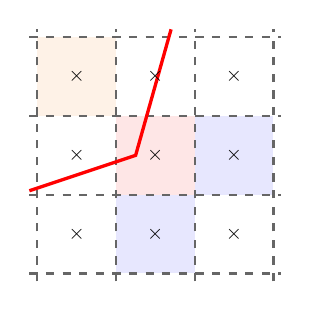
\begin{tikzpicture}[scale = 0.5, every node/.style={scale=0.5}]
			
\fill[red!95!gray!10] (2,2) rectangle (4,4);

\fill[blue!90!gray!10] (4,2) rectangle (6,4);
\fill[blue!90!gray!10] (2,0) rectangle (4,2);

\fill[orange!90!gray!10] (0,4) rectangle (2,6);

\foreach \x in { 0, 2, 4, 6}
    \draw[black!60, thick, dashed](-0.2,\x) -- (6.2,\x);

\foreach \x in { 0, 2, 4, 6}
   \draw[black!60, thick, dashed](\x,-0.2) -- (\x,6.2);


\draw[red, very thick] (3.4,6.2) -- (2.5,3) -- (-0.2, 2.1);

\foreach \x in { 1, 3, 5}
    \draw (1,\x) node[scale=1.5]{$\times$};
\foreach \x in { 1, 3, 5}
    \draw (3,\x) node[scale=1.5]{$\times$};
\foreach \x in { 1, 3, 5}
    \draw (5,\x) node[scale=1.5]{$\times$};

		\end{tikzpicture}

\end{center}
   \end{column}
   \end{columns}
\end{frame}


\begin{frame}
    \frametitle{Calcul du taux de transfert de masse par unité de surface}
	\footnotesize
On approche $\Dot{m}$ par : 
\begin{align} \label{eq:mPoint}
	\Dot{m} &= \frac{\lambda_l \, (\ghost T_l \cdot \norm) - \lambda_s \, (\ghost T_s \cdot \norm)}{\Delta \mathcal{H}^\Gamma}.
\end{align}
%où :
%\begin{align} \label{eq:mPointk}
%	\Dot{m}_k &= \lambda_k \, (\ghost T_k \cdot \norm),
%\end{align}

Pour assurer le respect de l'état de l'interface, si l'état est en conduction, alors, le taux $\Dot{m}$ est imposé à $0$.
\begin{align}
	\Dot{m} &= \left\{ {\renewcommand{\arraystretch}{2}\begin{array}{l l} 
	0 &\text{ si } E = \text{conduction},\\
	\frac{\lambda_l \, (\ghost T_l \cdot \norm) - \lambda_s \, (\ghost T_s \cdot \norm)}{\Delta \mathcal{H}^\Gamma} &\text{ sinon }.
	\end{array}}\right.	
\end{align}
\vspace{0.4cm}
\center\fbox{\begin{minipage}[]{0.8\textwidth}
\begin{center}
 \textcolor{red}{\textbf{Implémentation en 2D et 3D} de ces évolutions dans TrioCFD.\\
 	$\Rightarrow$ Validation et vérification.}
\end{center}
\end{minipage}}
\end{frame}




\begin{frame}
	\frametitle{Planification de validation}
	\footnotesize
	


	
	
\begin{columns}[c]
    \begin{column}{0.5 \textwidth}
    \color{cea_rouge}\underline{Cas test de Stefan 1D :}\color{cea_texte}\\
    	$\bullet$ Validation de l'adaptation de la méthode de pénalisation.\\
    	$\bullet$ Validation de l'adaptation de la méthode Ghost-Fluid.\\
    	


\end{column}
    \begin{column}{0.5 \textwidth}
		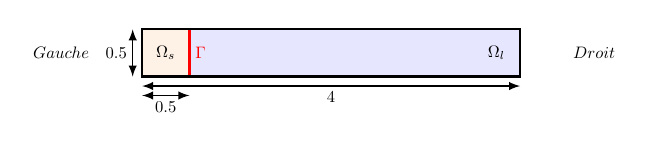
\begin{tikzpicture}[scale = 0.6, every node/.style={scale=0.6}]
			
\fill[orange!95!gray!10] (0,0) rectangle (1,1);
\fill[blue!95!gray!10] (1,0) rectangle (8,1);
\draw[red, very thick] (1,0) -- (1,1);

\draw (0.5, 0.5) node[ scale=1.]{$\Omega_s$};
\draw (7.5, 0.5) node[scale=1]{$\Omega_l$};


\draw[  thick] (0, 0.) rectangle(8, 1);

\draw[<->,>=latex] (0, -0.2) to (8, -0.2);
\draw[<->,>=latex] (0, -0.4) to (1, -0.4);
\draw[<->,>=latex] (-0.2, -0.) to (-0.2, 1);

\draw (.5, -0.4) node[scale=1, below]{$0.5$};
\draw (4, -0.2) node[scale=1, below]{$4$};
\draw (-0.2, 0.5) node[scale=1, left]{$0.5$};
\draw (1, 0.5) node[scale=1, right, red]{$\Gamma$};


\draw (-1, 0.5) node[scale=1, left]{$Gauche$};
\draw (9, 0.5) node[scale=1, right]{$Droit$};



		\end{tikzpicture}

   \end{column}
   \end{columns}	
   
   	
\begin{columns}[c]
    \begin{column}{0.5 \textwidth}
      \color{cea_rouge}\underline{Cas test de l'angle 2D \bib{Rathjen et al.} :}\color{cea_texte}\\
        $\bullet$ Validation de l'adaptation de la méthode de pénalisation.\\
    	$\bullet$ Validation de l'adaptation de la méthode Ghost-Fluid.\\
    	
\end{column}
    \begin{column}{0.5 \textwidth}
    		\center 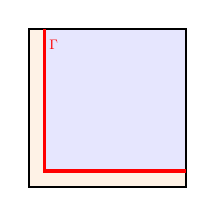
\begin{tikzpicture}[scale = 0.2, every node/.style={scale=0.2}]
			\fill[orange!95!gray!10] (0,0) rectangle (10,1);
\fill[orange!95!gray!10] (0,1) rectangle (2,10);
\fill[blue!95!gray!10] (1,1) rectangle (10,10);
    
\draw[ thick](10.,0) -- (10,10) -- (0,10) -- (0,0) -- cycle;
\draw[very thick, red] (1,10) -- (1,1)--(10,1);
%\draw (0.5,0.5) node[scale=1.5]{$\Omega_s$};
%\draw (9,9) node[scale=1.5]{$\Omega_l$};
\draw (1,9) node[scale=2.5, right, red]{$\Gamma$};












		\end{tikzpicture}


   \end{column}
\end{columns}	


	\begin{columns}[c]
    \begin{column}{0.5 \textwidth}
	\color{cea_rouge}\underline{ Cas test de la couche mince.}\color{cea_texte}\\
	$\bullet$ Résultats 2D.\\
	$\bullet$ Résultats 3D.
	
	\end{column}
    \begin{column}{0.5 \textwidth}
\center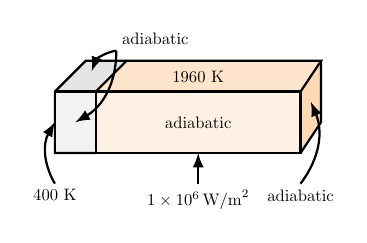
\begin{tikzpicture}[scale =0.26, every node/.style={scale=0.3}]

\fill[orange!10] (0,0) rectangle (10, 3);
\fill[orange!20] (0,3) -- (10, 3) -- (11, 4.5) -- (1.5, 4.5) -- cycle;
\fill[orange!30] (10, 3) -- (11, 4.5) -- (11, 1.5) -- (10,0) --cycle;
\fill[gray!10] (-2,0) rectangle (0, 3);
\fill[gray!20] (-2,3) -- (-0.5, 4.5) -- (1.5, 4.5) -- (0,3) -- cycle;

\draw[ thick, black] (0,0) rectangle (10, 3);
\draw[ thick, black] (10,3) -- (11, 4.5) -- (1.5, 4.5) -- (0,3);
\draw[ thick, black]  (11, 4.5) -- (11, 1.5) -- (10,0);
\draw[ thick, black]  (0, 0) -- (-2,0) -- (-2,3) -- (-0.5,4.5) -- (1.5, 4.5);
\draw[ thick, black]  (0, 3) -- (-2,3) ;

\draw (5,3.7) node[scale=2]{$1960$~K};
\draw (5,1.5) node[scale=2]{adiabatic};
\draw (1,5) node[scale=2, above right]{adiabatic};
\draw[->,>=latex, black, thick](1,5) to[bend right] (-0.2, 4);
\draw[->,>=latex, black, thick](1,5) to[bend left] (-1, 1.5);
\draw (-2,-1.5) node[scale=2, below]{$400$~K};
\draw[->,>=latex, black, thick](-2,-1.5) to[bend left]  (-2, 1.5);

\draw (5,-1.5) node[scale=2, below]{$1\times10^6\, \text{W/m}^2$};
\draw[->,>=latex, black, thick](5,-1.5) to (5, 0);


\draw (10,-1.5) node[scale=2, below]{adiabatic};
\draw[->,>=latex, black, thick](10,-1.5) to[bend right] (10.5, 2.5);



\end{tikzpicture}

   \end{column}
\end{columns}
\end{frame}



\begin{frame}
    \frametitle{Cas test de validation : cas test de Stefan}
	\scriptsize
\color{cea_rouge}\underline{Validation 1D de la méthode de pénalisation :}\color{cea_texte}\\
\begin{columns}
\begin{column}{0.5 \textwidth}

        %\vspace{0.5\linewidth}
        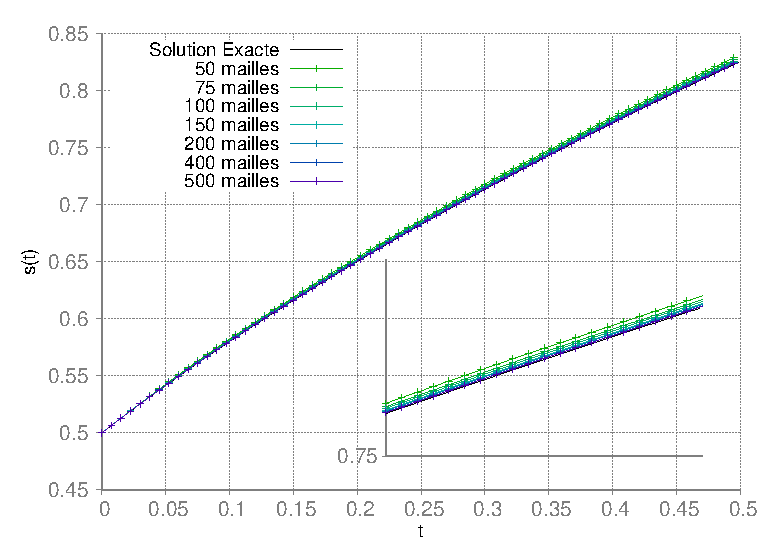
\includegraphics[width=1\textwidth]{Figures/StefanConvDX.eps}	
	%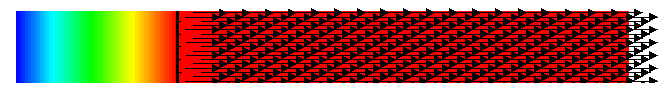
\includegraphics[width=1\textwidth]{Figures/avantApresRhoDiff0000.png}




\end{column}
    \begin{column}{0.5 \textwidth}
\begin{table}
	%    \hspace{-2cm}
	%\resizebox{.99\textwidth}{!}{
	%\renewcommand{\arraystretch}{1}
	\scriptsize
		\begin{tabular}{|c|c||cc|}
			\hline
			$N_x$ & $\Delta x$ & $L^2$ error & $L^2$ order \\
			\hline
			\hline
			50 	& 0.08  & $4.072E-3$ & --  \\
			75  & 0.053 & $2.752E-3$ & $0.95$  \\
			100 & 0.04  & $2.068E-3$ & $1.02$   \\
			150 & 0.027 & $1.368E-3$ & $1.05$   \\
			200 & 0.02  & $1.011E-3$ & $1.01$   \\
			400 & 0.01  & $5.137E-4$ & $0.98$   \\
			500 & 0.008 & $4.172E-4$ & $0.93$  \\
			\hline
			-- & --     &  $L^2$ average  $\rightarrow$ & 0.99 \\
			\hline
		\end{tabular}
\end{table}

   \end{column}
   \end{columns}

\center 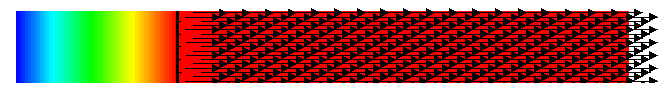
\includegraphics[width=0.8\textwidth]{Figures/avantApresRhoDiff0000.png}
\end{frame}
\begin{frame}
    \frametitle{Cas test de validation : cas test de Stefan}
	\scriptsize
	\color{cea_rouge}\underline{Validation 1D de la méthode Ghost-Fluid :}\color{cea_texte}\\
	\begin{center}

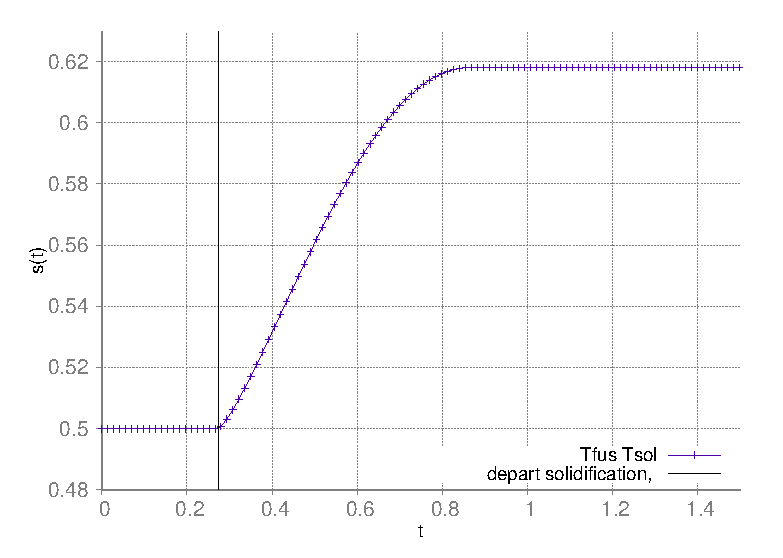
\includegraphics[width=0.85\textwidth]{Figures/StefanTFusTSol.eps}
\end{center}
	\end{frame}

\begin{frame}
    \frametitle{Cas test de validation : cas test de l'angle 2D}
	\footnotesize


\begin{columns}
\begin{column}{0.5 \textwidth}

\color{cea_rouge}\underline{Validation 2D de la méthode de pénalisation :}\color{cea_texte}\\
     \begin{center}
        %\vspace{0.5\linewidth}
        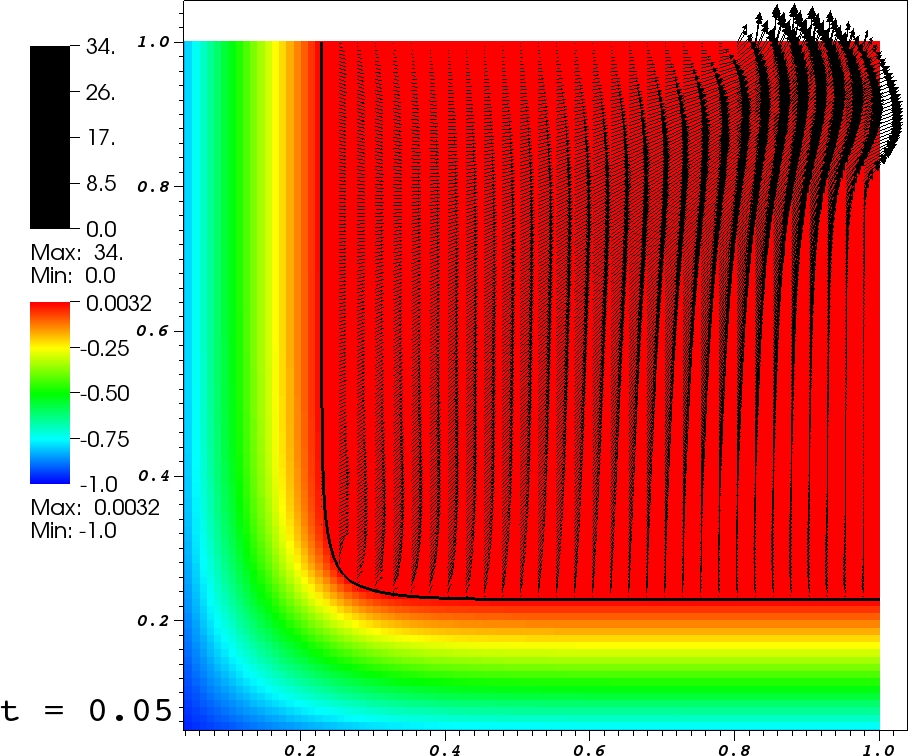
\includegraphics[width=1\textwidth]{Figures/angleIBCDiff0000.png}	

    \end{center}
\end{column}
    \begin{column}{0.5 \textwidth}
    \center 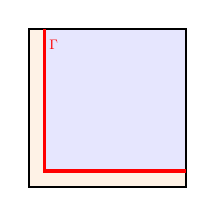
\begin{tikzpicture}[scale = 0.2, every node/.style={scale=0.2}]
			\fill[orange!95!gray!10] (0,0) rectangle (10,1);
\fill[orange!95!gray!10] (0,1) rectangle (2,10);
\fill[blue!95!gray!10] (1,1) rectangle (10,10);
    
\draw[ thick](10.,0) -- (10,10) -- (0,10) -- (0,0) -- cycle;
\draw[very thick, red] (1,10) -- (1,1)--(10,1);
%\draw (0.5,0.5) node[scale=1.5]{$\Omega_s$};
%\draw (9,9) node[scale=1.5]{$\Omega_l$};
\draw (1,9) node[scale=2.5, right, red]{$\Gamma$};












		\end{tikzpicture}
\begin{center}
	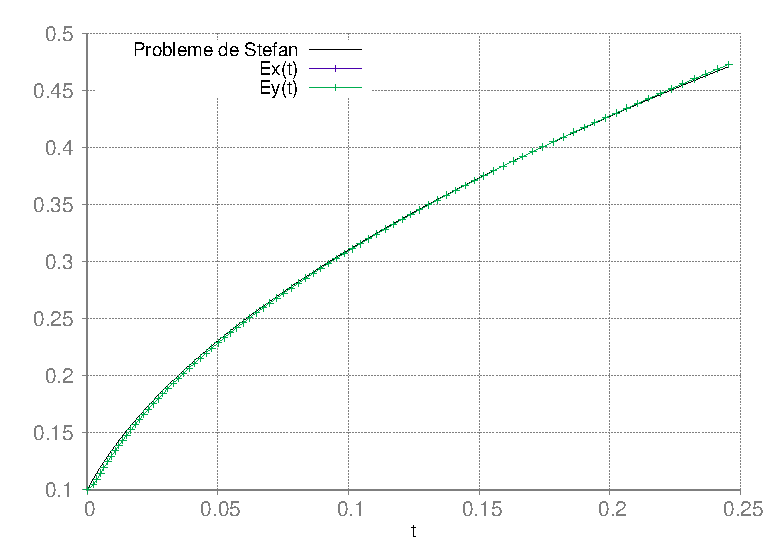
\includegraphics[width=0.7\textwidth]{Figures/AngleExEyDiff.eps}

\end{center}


   \end{column}
   \end{columns}


\end{frame}

\begin{frame}
    \frametitle{Cas test de validation : cas test de l'angle 2D}
    \footnotesize
\color{cea_rouge}\underline{Validation 2D de la méthode Ghost-Fluid :}\color{cea_texte}\\
\begin{center}

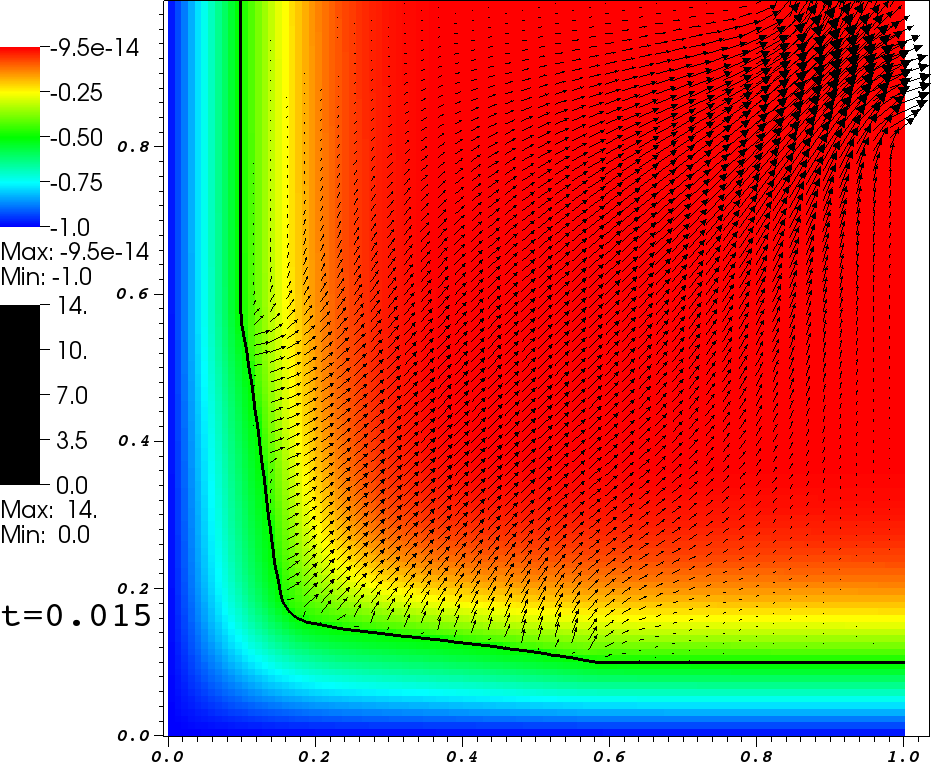
\includegraphics[width=0.7\textwidth]{Figures/AngleTfusTsol_0_0150000.png}
\end{center}

\end{frame}

\begin{frame}
    \frametitle{Cas test de la couche mince : présentation du cas test}
    \footnotesize
    % ---------   FIGURE   ---------------
\begin{figure}[h]
\centering
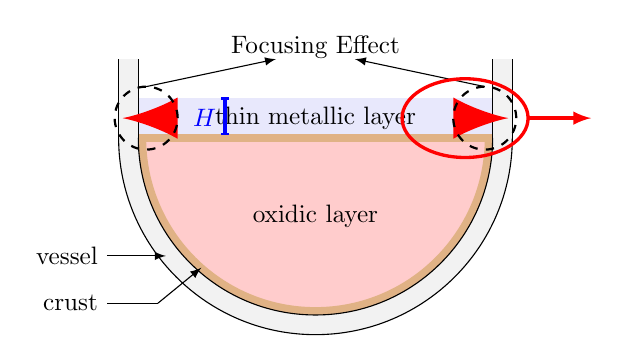
\begin{tikzpicture}[scale =0.5, every node/.style={scale=0.7}]

    
    %cuve
    \fill[gray!10] (0,2) -- (0,0)  arc (180:360:5) -- (10,2) -- (9.5,2) -- (9.5,0) arc (360:180:4.5) -- (0.5,2) -- cycle;
    
    %couche+croute
    \fill[red!20]  (0.5,0) arc (180:360:4.5) -- cycle;
    \fill[blue!80!gray!10](0.5,0) rectangle (9.5, 1);
    \fill[brown!80!orange!60] (0.5,0) arc (180:360:4.5) -- (9.3,0) arc (360:180:4.3) -- cycle;
    \fill[brown!80!orange!60](0.5,-0.1) rectangle (9.5,0.1);
    
    %cuve
    \draw (0,0) arc (180:360:5);
    \draw (0.5,0) arc (180:360:4.5);
    \draw (0,0) -- (0,2);
    \draw (0.5,0) -- (0.5,2);
    \draw (10,0) -- (10,2);
    \draw (9.5,0) -- (9.5,2);
    
    \draw (5,0.5) node[ scale=1.3]{thin metallic layer};
    \draw (5,-2) node[ scale=1.3]{oxidic layer};
    
    \draw[->,>=latex, red, line width = 2mm] (1.3, 0.5) to (0.1, 0.5);
    \draw[->,>=latex, red, line width = 2mm] (8.7, 0.5) to (9.9, 0.5);
    
    %FE
    \draw[black, dashed, thick] (0.7,0.5) circle (0.8);
    \draw[black, dashed, thick] (9.3,0.5) circle (0.8);
    \draw[->,>=latex] (0.7, 1.3) to (4, 2);
    \draw[->,>=latex] (9.3, 1.3) to (6, 2);
    \draw (5,2.3) node[ scale=1.3]{Focusing Effect};
    
    %cuve
    \draw[->,>=latex] (-0.3, -3) to (1.2, -3);
    \draw (-0.3, -3) node[ scale=1.3, left]{vessel};
    
    %croute
    
    \draw[->,>=latex] (1, -4.2) to (2.1, -3.3);
    \draw (1, -4.2) -- (-0.3, -4.2);
    \draw (-0.3, -4.2) node[ scale=1.3, left]{crust};


%convection
%\draw[->,>=latex] (1.6, -0.3) to[bend right=90] (1.6, -1.5);
%\draw[->,>=latex] (1.8, -2) to[bend right=90] (1.8, -0.3);

%\draw[->,>=latex] (3.6, -2) to[bend left=90] (3.6, -0.3);
%\draw[->,>=latex]  (3.8, -0.3) to[bend left=90] (3.8, -2);

%\draw[->,>=latex] (6.4, -2) to[bend right=90] (6.4, -0.3);
%\draw[->,>=latex]  (6.2, -0.3) to[bend right=90] (6.2, -2);


%\draw[->,>=latex] (8.4, -0.3) to[bend left=90] (8.4, -1.5);
%\draw[->,>=latex] (8.2, -2) to[bend left=90] (8.2, -0.3);

%\draw (4.5, -4.) -- (5.5, -4.);
%\draw (3.5, -3.5) -- (6.5, -3.5);
%\draw (2.5, -3.) -- (7.5, -3.);

%\draw[->,>=latex] (1.8, -2.5) to[bend right=20] (4.2, -4);
%\draw[->,>=latex] (8.2, -2.5) to[bend left=20] (5.8, -4);
\draw[blue, very thick] (2.7, 0.1) -- (2.7, 1);
\draw[blue,  thick] (2.6, 0.1) -- (2.8, 0.1);
\draw[blue,  thick] (2.6, 1) -- (2.8, 1);
\draw (2.7, 0.5) node[ scale=1.3, left, blue]{$H$};

\draw [red,  very thick](8.8,0.5) ellipse (1.6 and 1);
\draw[->,>=latex, very thick, red] (10.4, 0.5) to (12,0.5);
\end{tikzpicture}
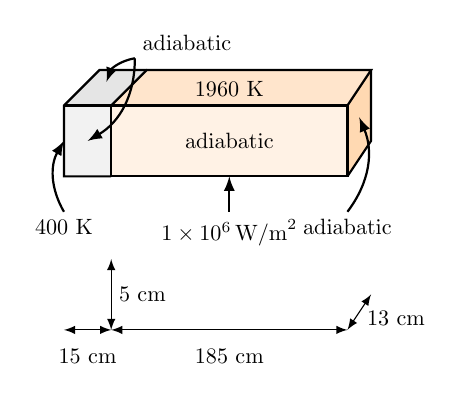
\begin{tikzpicture}[scale =0.3, every node/.style={scale=0.4}]

\fill[orange!10] (0,0) rectangle (10, 3);
\fill[orange!20] (0,3) -- (10, 3) -- (11, 4.5) -- (1.5, 4.5) -- cycle;
\fill[orange!30] (10, 3) -- (11, 4.5) -- (11, 1.5) -- (10,0) --cycle;
\fill[gray!10] (-2,0) rectangle (0, 3);
\fill[gray!20] (-2,3) -- (-0.5, 4.5) -- (1.5, 4.5) -- (0,3) -- cycle;

\draw[ thick, black] (0,0) rectangle (10, 3);
\draw[ thick, black] (10,3) -- (11, 4.5) -- (1.5, 4.5) -- (0,3);
\draw[ thick, black]  (11, 4.5) -- (11, 1.5) -- (10,0);
\draw[ thick, black]  (0, 0) -- (-2,0) -- (-2,3) -- (-0.5,4.5) -- (1.5, 4.5);
\draw[ thick, black]  (0, 3) -- (-2,3) ;

\draw (5,3.7) node[scale=2]{$1960$~K};
\draw (5,1.5) node[scale=2]{adiabatic};
\draw (1,5) node[scale=2, above right]{adiabatic};
\draw[->,>=latex, black, thick](1,5) to[bend right] (-0.2, 4);
\draw[->,>=latex, black, thick](1,5) to[bend left] (-1, 1.5);
\draw (-2,-1.5) node[scale=2, below]{$400$~K};
\draw[->,>=latex, black, thick](-2,-1.5) to[bend left]  (-2, 1.5);

\draw (5,-1.5) node[scale=2, below]{$1\times10^6\, \text{W/m}^2$};
\draw[->,>=latex, black, thick](5,-1.5) to (5, 0);


\draw (10,-1.5) node[scale=2, below]{adiabatic};
\draw[->,>=latex, black, thick](10,-1.5) to[bend right] (10.5, 2.5);


\draw[<->,>=latex] (0, -3.5) to (0, -6.5);
\draw[<->,>=latex] (0, -6.5) to (10, -6.5);
\draw[<->,>=latex] (10, -6.5) to (11, -5.);
\draw[<->,>=latex] (0, -6.5) to (-2, -6.5);

\draw (5,-7) node[scale=2, below]{$185$~cm};
\draw (10.5,-6) node[scale=2, right]{$13$~cm};
\draw (-1,-7) node[scale=2, below]{$15$~cm};
\draw (0,-5) node[scale=2, right]{$5$~cm};

\end{tikzpicture}
\label{fig:configCoucheMince}
\end{figure}
% ---------   FIGURE   ---------------


\begin{table}[!h]
	\centering
	\tiny
		\begin{tabular}{|c|c|}
		\hline
		Parameter & Value\\
		\hline \hline
		Density $\rho$ & $6720$~$\text{kg/m}^3$\\	
		Coefficient of thermal expansion, $\beta$ & $3\times 10^{-5}$\\
		Thermal conductivity, $\lambda$ & $20$~W/mK\\
		Fusion temperature, $T^\fus$ & $1658$~K\\
		Enthalpy of fusion, $\Delta \mathcal{H}^\fus$ & $2.76\times 10^5$~J/kg\\
		Heat capacity, $C_p$ & $674$~J/kg~K\\
		Kinematic viscosity, $\mu$ & $4.5696 \times 10^{-3}$~$\text{m}^2/\text{s}$\\
		\hline
		\end{tabular}%}
	\label{tab:Acier}
\end{table}
\end{frame}

\begin{frame}
    \frametitle{Résultat 2D}
    \footnotesize
\begin{columns}[c]
    \begin{column}{0.5 \textwidth}
\begin{center}
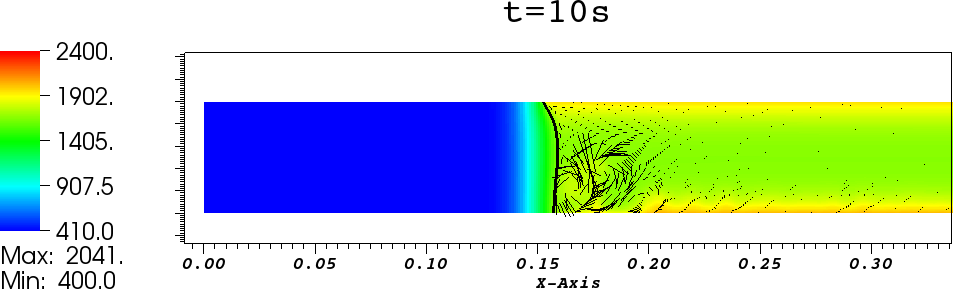
\includegraphics[width=0.9\textwidth]{Figures/CoucheMince0100000.png}\\
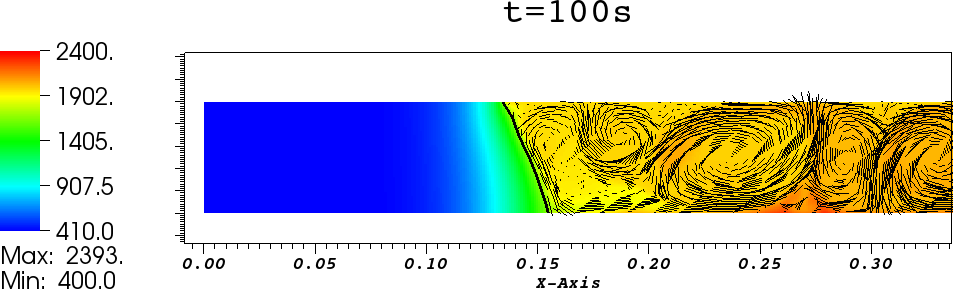
\includegraphics[width=0.9\textwidth]{Figures/CoucheMince1000000.png}\\
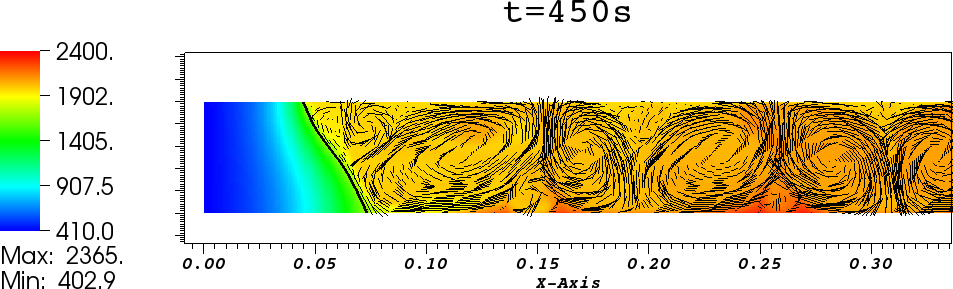
\includegraphics[width=0.9\textwidth]{Figures/CoucheMince4500000.png}


\end{center}
\end{column}
    \begin{column}{0.5 \textwidth}
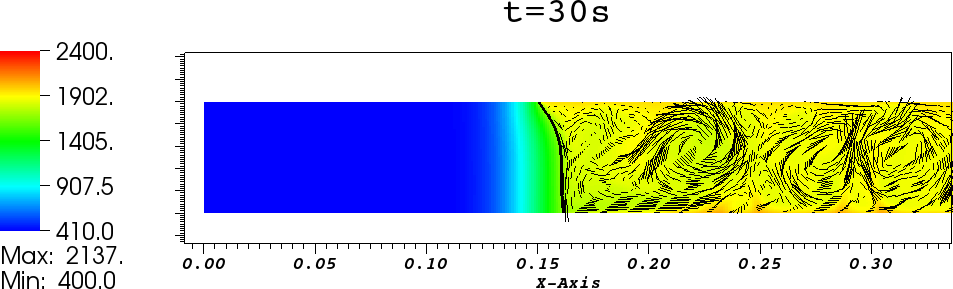
\includegraphics[width=0.9\textwidth]{Figures/CoucheMince0300000.png}\\
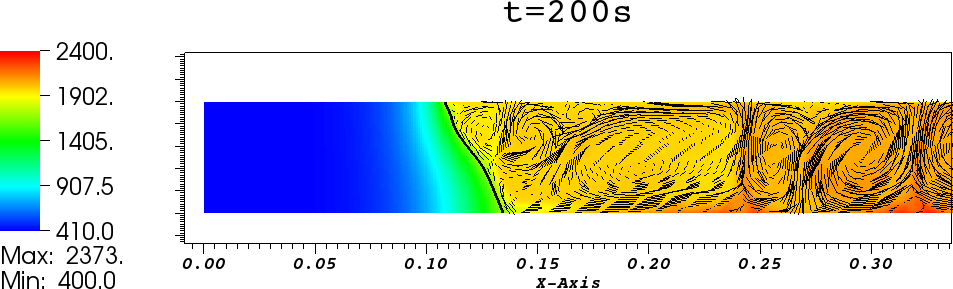
\includegraphics[width=0.9\textwidth]{Figures/CoucheMince2000000.png}\\
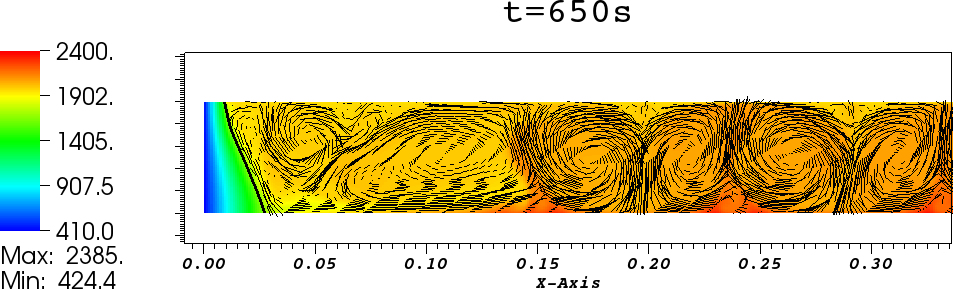
\includegraphics[width=0.9\textwidth]{Figures/CoucheMince6500000.png}

   \end{column}
   \end{columns}
\center Cas test de la couche mince 2D -- Température (couleur), vitesse (vecteurs noirs) et interface (trait noir).

\end{frame}

\begin{frame}
    \frametitle{Résultat 3D}
    \scriptsize


\begin{columns}[c]
    \begin{column}{0.5 \textwidth}
\begin{center}
   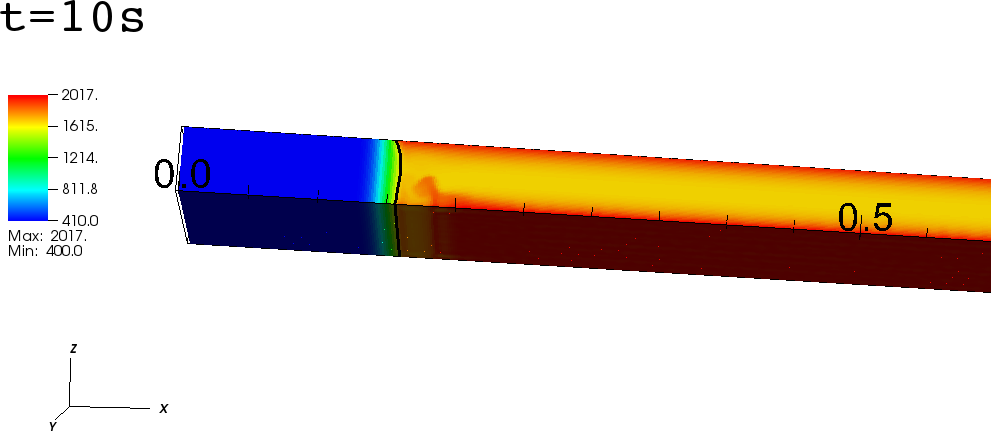
\includegraphics[width=0.7\textwidth]{./Figures/10s_TEMP0000.png}\\
	\hspace{-0.8cm}
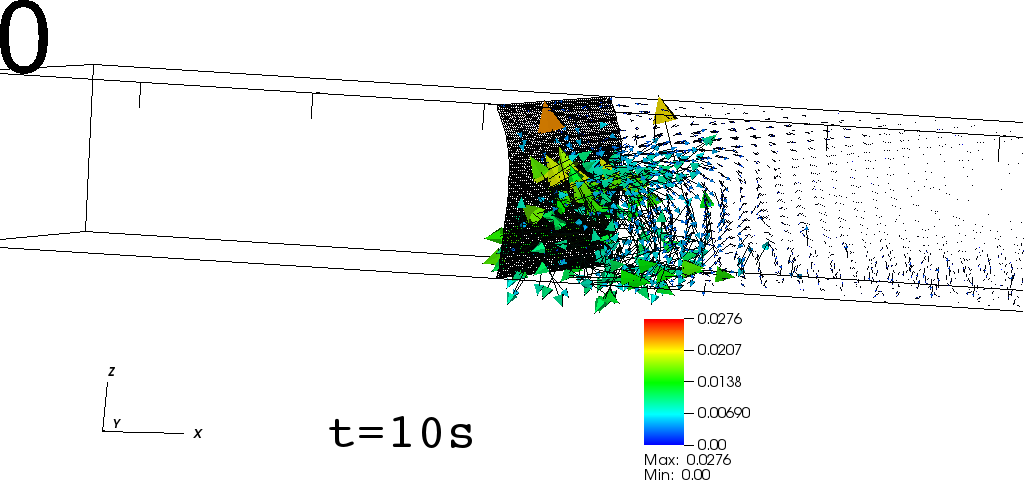
\includegraphics[width=0.7\textwidth]{./Figures/10s_VIT0000.png}\\
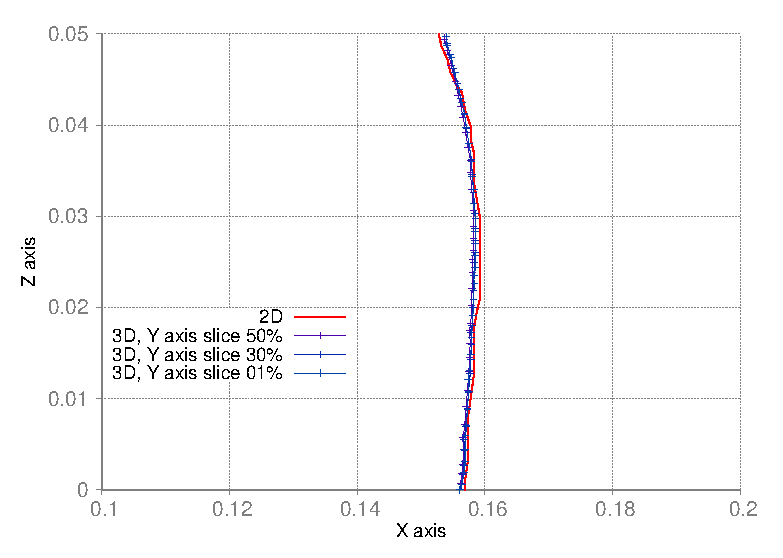
\includegraphics[width=0.6\textwidth]{./Figures/PositionInterface3D_10s.eps}


\end{center}
\end{column}
    \begin{column}{0.5 \textwidth}
\begin{center}
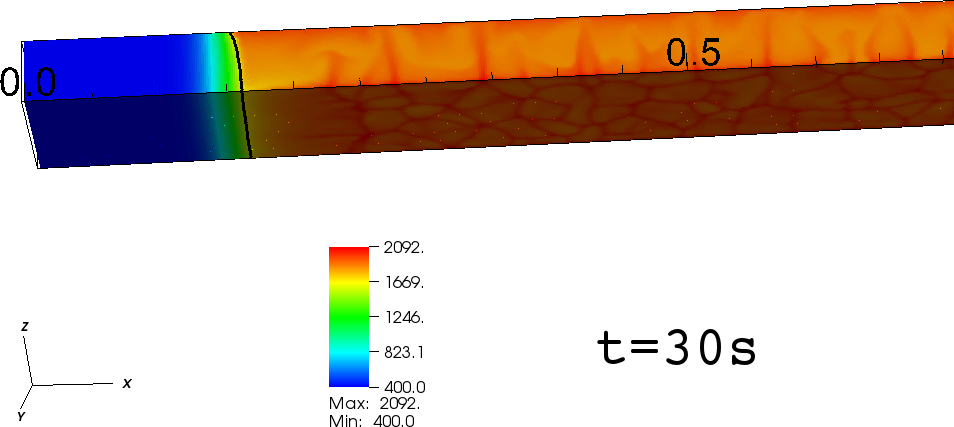
\includegraphics[width=0.7\textwidth]{./Figures/CoucheMinceTEMP0300001.png}\\
\hspace{-0.8cm}
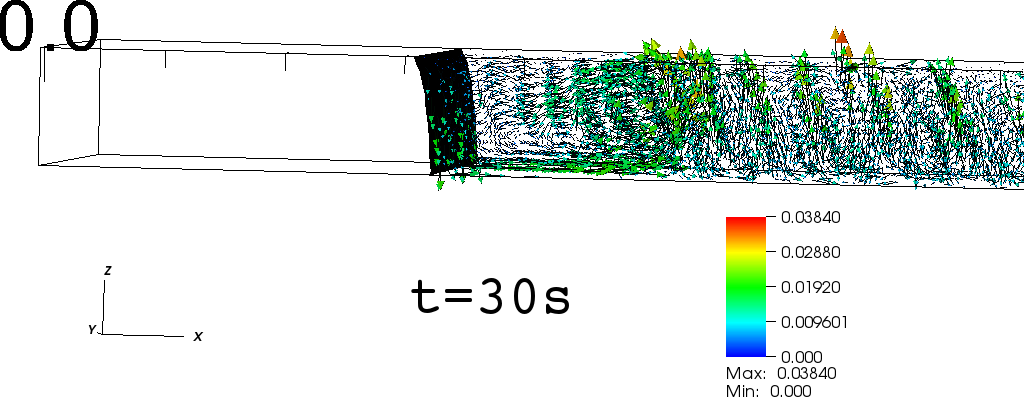
\includegraphics[width=0.7\textwidth]{./Figures/CoucheMinceVIT0300000.png}\\
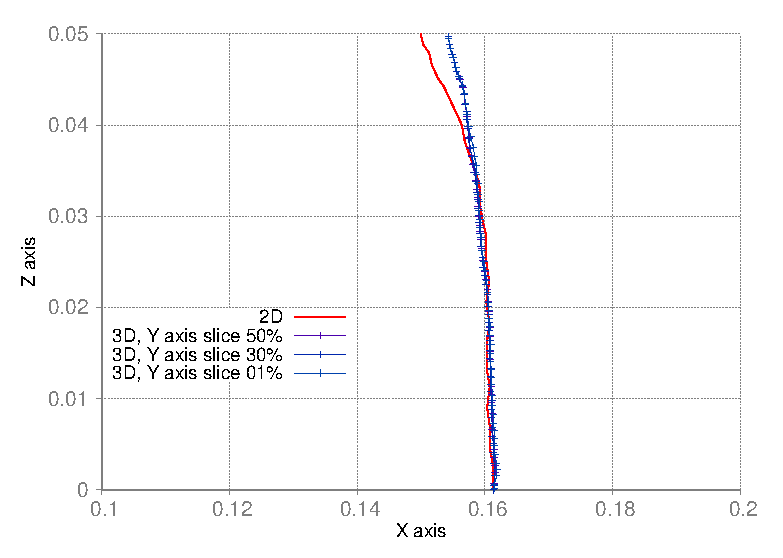
\includegraphics[width=0.6\textwidth]{./Figures/Yslice_30s.eps}


\end{center}
   \end{column}
   \end{columns}
\center Cas test de la couche mince 3D -- En haut : température en couleur -- Au milieu : vecteur vitesse  -- En bas : comparaison entre la position de l'interface pour plusieurs coupes et avec le résultat 2D.


\end{frame}


%--------------------------------------------------------------------------
%==========================================================================
%--------------------------------------------------------------------------
\section{Conclusions et perspectives}
\Intercalaire{Conclusions et perspectives}

\begin{frame}
    \frametitle{Conclusions}
    \scriptsize
    \begin{ceablock}{Modèle 2D lagrangien du code \procor}
        \begin{itemize}
            \item Un nouveau modèle 2D a été développé. L'équation de la chaleur est résolue en 2D et l'interface liquide-solide évolue en 2D.
            \item Méthode éléments finis mixtes, remaillage, projection.
            \item Possibilité de couplage du modèle 2D avec les modèles 0D de la plateforme \procor{}.
            \item Validations : académiques et comparaisons.
            \item Cas test semi-industriel (formation de la croûte), avec comparaison au modèle 0D.
        \end{itemize}
    \end{ceablock}
    
     \begin{ceablock}{Modèle CFD dans le code TrioCFD}
        \begin{itemize}
        	\item Définition de la notion d'états d'interface et écriture d'un modèle CFD  adapté.
            \item Adaptation d'une méthode VOF-FT à notre problématique liquide solide.
            \item Adaptation de la méthode de pénalisation pour supprimer la vitesse sur le solide.
            \item Adaptation de la méthode Ghost-Fluid pour prendre en compte les différentes fermetures thermique de l'interface.
            \item Validation des développements réalisés sur des cas tests 1D, 2D et 3D.
            \item Simulation du cas test de la  couche métallique légère, simulation 2D et 3D.
        \end{itemize}
    \end{ceablock}

\end{frame}


%\begin{frame}
%    \frametitle{Perspectives pour le modèle 2D lagrangien}
%    \scriptsize
%    \color{cea_rouge}\underline{Validation :} \color{cea_texte}
%         \begin{itemize}
%        	\item  Poursuite de la validation du modèle 2D développé dans \procor, notamment avec une comparaison entre code maillé.
%        	\end{itemize}
%        	\color{cea_rouge}\underline{Utilisation future des développements :} \color{cea_texte}
%        	\begin{itemize}
%        	 \item  Utilisation du modèle dans d'autres applications, par exemple pour la modélisation d'un récupérateur dans le cadre d'un réacteur neutron rapide.
        	 
        	  
            
%        \end{itemize}
        	
%        	\color{cea_rouge}\underline{Complexification de la modélisation :} \color{cea_texte}
%        \begin{itemize}
%        	\item  Complexification de la physique à l'interface, par exemple en prenant en compte un changement de phase non congruent et en introduisant des modèles de thermochimie.
%        	\end{itemize}
        	

%\end{frame}

\begin{frame}
\setlength{\columnseprule}{0.5pt}
    \frametitle{Perspectives}
    \scriptsize

    \begin{multicols}{2}
    
	\center \fcolorbox{black}{cea_grisclair}{\begin{minipage}[]{0.4\textwidth}
 \center\textcolor{red}{Modèle 2D lagrangien}
\end{minipage}}
        
\columnbreak
			
			\center \fcolorbox{black}{cea_grisclair}{\begin{minipage}[]{0.4\textwidth}
 \center\textcolor{red}{Modèle CFD}
\end{minipage}}

\end{multicols}
    \center\color{cea_rouge}\underline{Validation et vérification :} \color{cea_texte}\\
\begin{multicols}{2}
        \begin{itemize}
        
        
        \item Vérification par  comparaison avec d'autre modèles maillés.
        \end{itemize}
        
\columnbreak
			
		
        \begin{itemize}
        
        
        \item Validation 3D de la méthode Ghost-Fluid.
			\item Benchmark : essais LIVE, collaboration.
        \end{itemize}
		
\end{multicols}
\center\color{cea_rouge}\underline{Utilisation future des développements :} \color{cea_texte}
\begin{multicols}{2}
        \begin{itemize}
        
        
        \item Modélisation d'un récupérateur.
        \end{itemize}
        
\columnbreak
			
		
        \begin{itemize}
        
        
        \item Étude de la couche mince.
        \end{itemize}
		
\end{multicols}

\center\color{cea_rouge}\underline{Complexification de la modélisation :} \color{cea_texte}
\begin{multicols}{2}
        \begin{itemize}
        
        
        \item Modèle de thermochimie à l'interface.
        \item Changement de phase non congruent.
        \end{itemize}
        
\columnbreak
			
		
        \begin{itemize}
        
        \item Ajout de méthode LES.
        \item Remplacement du Ghost-Fluid.
        \item Introduction du suivi des espèces.
        \end{itemize}
		
\end{multicols}



\end{frame}





%\begin{frame}
%    \frametitle{Perspectives pour le modèle VOF-FT}
%    \scriptsize
%        \color{cea_rouge}\underline{Validation :} \color{cea_texte}
%         \begin{itemize}
        	
        	  	
%        	\item  Validation 3D de la méthode Ghost-Fluid adaptée. Plus largement, des benchmarks entre codes et méthodes numériques pour valider les développements réalisés sur la méthode VOF-FT. 
%        	        	\end{itemize}
%        	        	\color{cea_rouge}\underline{Utilisation future des développements :} \color{cea_texte}
%        \begin{itemize}
%        	\item Benchmark avec d'autres codes liée à une campagne d'essais LIVE.
%        	\item Prochaine collaboration avec des équipes canadiennes sur un benchmark portant sur une configuration 3D.
%        	\item Poursuite de l'étude de la couche mince avec ajout de méthodes LES (Large Eddy Simulation) pour la modélisation de la turbulence.
        	
%        	\end{itemize}
%        	\color{cea_rouge}\underline{Complexification de la modélisation :} \color{cea_texte}
%        	\begin{itemize}
            
%            \item Amélioration de la méthode d'interpolation utilisée dans la méthode Ghost-Fluid. Éventuellement remplacement de la méthode Ghost-Fluid pour une méthode plus adaptée.
%            \item Introduction du suivi des espèces dans le modèle de CFD.
            
           
%            \end{itemize}
%        	\color{cea_rouge}\underline{Lien entre CFD et modèles intégraux :} \color{cea_texte}
%        	\begin{itemize}
            
           
%            \item Proposer des remontées d'échelles entre les simulations CFD et les modélisations intégrales.
            
            
%        \end{itemize}

%\end{frame}

%--------------------------------------------------------------------------
%==========================================================================
%--------------------------------------------------------------------------
%\section{Bibliographie}
\Intercalaire{Bibliographie}
%------------------------------------------------------------------------------------------galium3minBIS0000

\begin{frame}
    \frametitle{Bibliographie}
	\scriptsize
\color{cea_rouge}\underline{Bibliographie \procor{} :} \color{cea_texte}
\begin{itemize}
	\item Viot, L., Saas, L., De Vuyst, F., 2018. \textbf{Solving coupled problems of lumped parameter models in a platform for severe accidents in nuclear reactors.} International Journal for Multiscale Computational Engineering.
	\item Le Tellier, R., Skrzypek, E., Saas, L., 2017. \textbf{On the treatment of plane fusion front in lumped parameter thermal models with convection.} Applied Thermal Engineering 120, 314–326. 
	\item \url{https://fenicsproject.org/} 
	\item Viot, L., Le Tellier, R., Peybernes, M., 2020. \textbf{Modeling of the corium crust of a stratified corium pool during severe accidents in light water reactors.} Nuclear Engineering and Design.
	\item \color{blue} Drouillet, A., Le Tellier, R., Loubère, R., Peybernes, M., Viot, L., 2021. \textbf{Multi-dimensional simulation of phase change by a 0D-2D model coupling via Stefan condition.} Communications on Applied Mathematics and Computation.

\end{itemize}
\color{cea_rouge}\underline{Bibliographie TrioCFD :} \color{cea_texte}


\begin{itemize}
	\item \url{https://triocfd.cea.fr/}
	\item Mathieu, B., n.d. \textbf{Études physique, expérimentale et numérique des mécanismes de base intervenant dans les écoulements diphasiques en micro-fluidique.} Polytech Marseille.
	\item Bois, G., 2021. \textbf{A comprehensive description of the mixed Front-Tracking/Volume-of-Fluid/Level-set algorithm of TrioCFD.} (preprint)
	\item Belliard, M., Fournier, C., 2010. \textbf{Penalized direct forcing and projection schemes for Navier–Stokes.} Comptes Rendus Mathematique 348, 1133–1136.
	\item \color{blue} Drouillet, A., Bois, G., Le Tellier, R., Loubère, R., Peybernes, M.,  \textbf{Mathematical modeling and associated numerical simulation of fusion/solidification front evolution in the context of severe accident of nuclear power engineering.} En revision mineure dec. 2021.
 

\end{itemize}
\end{frame}





\begin{frame}[noframenumbering]
    \frametitle{Bibliographie}
	\tiny
%ÉTUDES PHYSIQUE, EXPÉRIMENTALE ET NUMÉRIQUE DES MÉCANISMES DE BASE INTERVENANT DANS LES ÉCOULEMENTS DIPHASIQUES EN MICRO-FLUIDIQUE
\begin{itemize}
	\item \bib{Jacquemain et al.} Bentaïb, A., Jacquemain, D., 2013. \textbf{Les accidents de fusion du coeur des réacteurs nucléaires de puissance: état des connaissances}, Collection sciences et techniques. EDP sciences, Les Ulis.

	\item \bib{Tsurikov et al.} D.F. Tsurikov, V.F. Strizhov, S.V. Bechta, V.N. Zagriazkin, and N.P. Kiselev. \textbf{Main results of masca 1 and 2 projects.} RRC Kurchatov Institute, Technica report, 2007.
	\item \bib{Gupta} S.C. Gupta. \textbf{Chapter 1 - the stefan problem and its classical formulation.} The Classical Stefan Problem (Second Edition), pages 1 – 35, 2018.
	\item \bib{Stefan} J. Stefan. \textbf{Uber die theorie der eisbildung.} Monatshefte Mat. Phys., 1 :1–6, 1890.
	\item \bib{Viot et al. 2018} Viot, L., Saas, L., De Vuyst, F., 2018. \textbf{Solving coupled problems of lumped parameter models in a platform for severe accidents in nuclear reactors.} International Journal for Multiscale Computational Engineering.
	\item \bib{Le Tellier et al.} Le Tellier, R., Skrzypek, E., Saas, L., 2017. \textbf{On the treatment of plane fusion front in lumped parameter thermal models with convection.} Applied Thermal Engineering 120, 314–326.
	\item \bib{Project Fenics} \url{https://fenicsproject.org/}
	\item \bib{Rathjen et al.} K.A. Rathjen and L.M. Jiji. \textbf{Heat conduction with melting or freezing in a corner.}
ASME. J. Heat Transfer, 93 :101–109., 1971.
	\item \bib{Viot et al. 2020} Viot, L., Le Tellier, R., Peybernes, M., 2020. \textbf{Modeling of the corium crust of a stratified corium pool during severe accidents in light water reactors.} Nuclear Engineering and Design.
	\item \bib{TrioCFD} \url{https://triocfd.cea.fr/}
	\item \bib{Benson} David J Benson. \textbf{Volume of fluid interface reconstruction methods for multi-material
problems.} Applied Mechanics Reviews, 55(2) :151–165, 04 2002.
	\item \bib{Tryggvason et al.} G. Tryggvason, B. Bunner, A. Esmaeeli, D. Juric, N. Al-Rawahi, W. Tauber, J. Han,
S. Nas, and Y.-J. Jan. \textbf{A front-tracking method for the computations of multiphase flow.} Journal of Computational Physics, 169(2) :708–759, 2001.
	\item \bib{Belliard et al.} Belliard, M., Fournier, C., 2010. \textbf{Penalized direct forcing and projection schemes for Navier–Stokes.} Comptes Rendus Mathematique 348, 1133–1136.

\end{itemize}


\end{frame}
%==========================================================================================
\Intercalaire{Merci pour votre attention}
\end{document}
